% Useful packages
\documentclass[12pt]{article}
\usepackage[a4paper,top=3.5cm,bottom=3.5cm,left=2.8cm,right=2.8cm,marginparwidth=1.75cm]{geometry}
\usepackage[colorlinks=false, allcolors=blue]{hyperref}
\usepackage[format=plain,
            font=it]{caption}


%---spacing---
\usepackage{titlesec}
\titlespacing*{\section}
{0pt}{4ex plus 1ex minus .2ex}{3ex plus .2ex}
\titlespacing*{\subsection}
{0pt}{4ex plus 1ex minus .2ex}{3ex plus .2ex}
\titlespacing*{\subsubsection}
{0pt}{4ex plus 1ex minus .2ex}{3ex plus .2ex}

%---math---
\usepackage{float}
\usepackage{amsmath, amssymb}
\DeclareMathOperator{\EX}{\mathbb{E}}% expected value
\DeclareMathOperator{\ZX}{\mathbb{Z}}% expected value

%--extra utility--
\usepackage{minted} % Per i JSON e python
\usepackage{graphicx}
\usepackage{xcolor} %per i colori

%---date---
\usepackage{datetime}
\newdateformat{monthyeardate}{%
  \monthname[\THEMONTH], \THEYEAR}
  
%---biblio---
\usepackage[sorting=none]{biblatex} %Imports biblatex package
\addbibresource{sample.bib} %Import the bibliography file


%---- deleted packages ----
%\usepackage{blindtext}
%\usepackage[T1]{fontenc}
%\usepackage[utf8]{inputenc}
%\usepackage[colorlinks=true, allcolors=blue]{hyperref}
%\usepackage{dsfont}
%\usepackage{authblk}
%----------------

\begin{document}

%----------------------------------------------------------------------
%	TITLE PAGE
%-----------------------------------------------------------------------
%%%% Title Page


\begin{titlepage}

\newcommand{\HRule}{\rule{\linewidth}{0.3mm}} 							% horizontal line and its thickness
\center 

\vspace*{15mm} 
% University
\text{\large {ALMA MATER STUDIORUM - UNIVERSITÀ DI BOLOGNA}}\\[0.3cm]
\HRule \\[0.4cm]
\textsf{Master in Artificial Intelligence - Deep Learning course}\\[2cm]

% Document info

{ \huge\textbf{Flatland Project} }\\[1.5cm]							
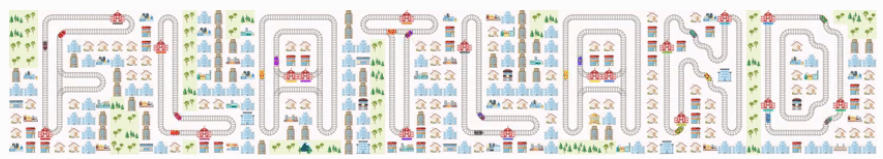
\includegraphics[scale=0.50]{res/title.png}\\[1cm] 
\textsf{Marco Cucè, Alessandro Stockman, Alessandra Stramiglio}\\
\vspace{8cm}
\vfill

\textit{Academic Year 2020/2021} 


\end{titlepage}


\tableofcontents
\newpage


\section{Introduction}

Flatland \cite{flatland-challenge} is a challenge organized by AIcrowd in collaboration with the Swiss Federal Railways (SBB) aimed at managing dense traffic on complex railway networks in an efficient way.

It represents a real-world problem faced by many transportation and logistics companies. The goal of the challenge is to plan the path of an arbitrary number of trains inside a rail environment by guiding them towards a target station with minimal travel time by minimizing the number of steps that it takes for each agent to reach its destination. 

The purpose of this work is to find a solution using modern Reinforcement-Learning approaches.  

\subsection{Reinforcement Learning}\label{RL}
\textbf{Reinforcement Learning} (RL) is one of the three main Machine Learning methods (Supervised Learning, Unsupervised Learning, Reinforcement Learning). RL lies in between full supervision and complete lack of predefined labels. On one hand, it uses well-known methods of supervised learning, such as \textbf{deep neural networks} for function approximation, stochastic gradient descent and backpropagation to learn data representation. On the other hand, RL applies those methods in a different way.  The key components of RL are the \textbf{Agent}, the \textbf{Environment} and \textbf{Rewards}.

\begin{itemize}
    \item 
    The \textbf{reward} is a scalar value obtained periodically from the environment representing the quality of the agent's behaviour. The frequency of the reward is not predefined, but it's common practice to set it to a fixed timestamp or at every environment interaction. The term \textit{reinforcement} derives, indeed, from the fact that reward obtained by an agent should reinforce its behaviour in a positive or negative way. Reward is \textit{local}, it reflects the success of the agent's recent activity and not all the successes achieved by the agent so far.
        
    \item 
    The \textbf{agent} is somebody or something that interacts with the environment by executing certain actions based on reasoning on observations and therefore receiving rewards for this. In practical scenarios, the agent is a portion of software that is supposed to solve some problem in an ideally efficient way. 
        
    \item 
    The \textbf{environment} represent everything outside of an agent. The agent's communication with the environment is limited to reward (obtained from the environment), actions (executed by the agent) and observations (information the agent receives about the environment).
    
\end{itemize}

\begin{figure}[H]
        \centerline{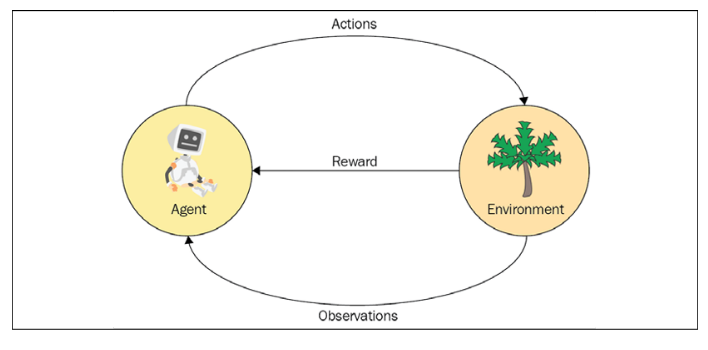
\includegraphics[scale=.45]{res/rl.png}}
        \caption{Graphical representation of RL entities and their communication channels.}
\end{figure}

The agent performs \textbf{actions} in the environment which can be either discrete or continuous: the former being a set of mutually exclusive interactions that an agent can perform and the latter involving continuous values. 

The state of an environment differs from the agent's view by including every detail about the environment itself, while the observation represents what the agent perceives about it. A temporal sequence of environment's states is usually called \textit{episode}.

\subsubsection{Markov Decision Process}
Markov Decision Process (MDP) is used to formulate any problem in RL mathematically. In the \textbf{Markov Process Chain},  $X_t$ represents the state of the process at time \textit{t}, with $t \in \ZX^+$. Each move from state \textit{i} to \textit{j} in one time-step has a \textit{transition probability} $p_{ij}$. This probability is fixed, i.e. it does not change over time. 

This process defined above has the property that the probability of moving from some state \textit{i} to another state \textit{j} is independent of the states visited prior to \textit{i}.
            \[ P(X_{t+1} = j|X_t=i, X_{t-1}=i_{t-1},...,X_1=i_1,X_0=i_0) = P(X_{t+1} = j|X_t=i) = p_{ij}\]

The transition probability can be captured by a transition matrix, which is a \textit{NxN} matrix, where \textit{N} is the number of states in our model and the row index \textit{i} represents the source state and the column \textit{j} represents the target state and each cell is equivalent to the probability to go from the source state to the target state.

In Reinforcement learning, the goal is maximizing the cumulative reward (all the rewards agent receives from the environment) instead of, the reward agent receives from the current state (also called immediate reward). Adding reward to the Markov Chain leads to the \textbf{Markov Reward Process}. Each reward is multiplied by a discount factor $\gamma$ in order to weight the importance of the immediate and future rewards. This total sum of reward the agent receives from the environment, is called \textit{return} and is defined as follows.
\[G_t = R_{t+1} + \gamma R_{t+2} + ...= \sum^\infty_{k=0} \gamma^k R_{t+k+1}\]

It follows that a Markov Reward Process is a Markov chain with values judgement. Basically, a value is obtained from every state our agent is in. Mathematically, a Markov Reward Process is defined as $R_s = \EX[R_{t+1}|S_t]$.

The last step to obtain the MDP is to add agent's actions. The Markov Process and Markov Reward Process had transition matrix, able to express the probability to jump from a source state to a target state. Hence, the agent is able to choose an action to take at every state transition, the 2D matrix becomes 3D matrix where the depth is governed by the possible actions the agent can perform to reach the target state from the source state.

\subsubsection{Policy}

The policy is the core concept in which Reinforcement Learning is built around, it is defined by the set of rules controlling the agent's behaviour.
The main objective of RL is to obtain as much \textbf{return} as possible and different policies can provide different amounts of return, therefore, the ideal goal is to find the \textit{optimal policy} for the agent. 

Formally, policy is defined as the probability distribution over actions for every possible state:
\[ \pi(a|s) = P[A_t=a|S_t=s]\]

\subsubsection{Bellman Equation}

Optimal policies are really hard to formulate and it's even harder to prove their optimality. Intuitively a policy could contain "greedy" features.
Bellman Equation is used to find optimal policies and value function. The policy changes with experience therefore, the value function will differ based on the policies. Optimal value function is one which gives maximum value compared to all other value functions.

The value of the state is $V(s)=\EX[\sum^\infty_{t=0} r_t\gamma^t]$, where $r_t$ is the local reward obtained at a step \textit{t} of the episode.

The total reward could be discounted with $\gamma$ or not (undiscounted case equals to $\gamma=0$). The value is always calculated in terms of some policy that the agent follows.

To introduce this concept it's better to start by putting ourselves into a deterministic case, where all actions have a 100\% guaranteed outcome. Assume that the agent observes state $s_0$ and has \textit{N} available actions, every action leads to another state $s_1,...,s_N$ with respective reward, $r_1,...,r_N$. Also, assume that the values $V_i$ of all states connected to state $s_0$ are known. The best course of action that the agent can take in such state is:
\[ V_0 = max_{a \in 1...N} (r_a+ \gamma V_a)\]

In this equation also the long-term value of the state is considered. Bellman proved that with this extension, the behaviour will get the best possible outcome, in other words, it will be optimal. The above equation is called the Bellman equation of value. 

In addition to the value of the state, \textit{V(s)}, it's convenient to introduce the value of the action, \textit{Q(s,a)}. It represent the total reward the agent can get by executing action \textit{a} in state \textit{s} and can be defined via \textit{V(s)}. Even if it is a less fundamental entity than \textit{V(s)}, this quantity gave a name to a whole family of methods called \textbf{Q-learning}. In this methods, our primary objective is to get values for Q for every pair of state and action.

\textit{V(s)} can also be  written via \textit{Q(s,a)}:
\[V(s,a)= max_{a\in A}Q(s,a)\]

This means that the value of some state equals to the value of the maximum action the agent can execute from this state. \textit{Q(s,a)} results as follows:
\[Q(s,a) = r(s,a) + \gamma max_{a' \in A} Q(s',a')\]

Q-values are much more convenient in practice, as for the agent, it's much simpler to make decisions about actions based on Q than on V. In the case of Q, to choose the action based on the state, the agent just need to calculate Q for all available actions using the current state and choose the action with the largest value of Q. To do the same using values of the states, the agent needs to know not only values, but also probabilities for transitions. In practice they are rarely known in advance, so the agent needs to estimate transition probabilities for every action and state pair.

\subsubsection{Multi-Agent Reinforcement Learning}
Often the multi-agent case is often reflected into real cases, where several agents are involved in the environment interaction. Of course, those agents can communicate between each other, in terms of communication it's possible to define two groups of agents:
\begin{itemize}
    \item Competitive: When two or more agents try to beat each other in order to maximize their reward (chess, Atari pong etc.)
    \item Collaboration: When a group of agents need to use joint efforts to reach the goal.
\end{itemize}

In multi-agent case, most of the elements are dependent of all the agents:
\begin{itemize}
    \item The state transitions are the result of the joint action of all the agents.
    \item The rewards of the agents depend on the joint action.
    \item Their returns depend on the joint policy.
    \item The Q-function of each agent depends on the joint action and on the joint policy.
\end{itemize}

In fully cooperative stochastic problems, the reward functions are the same for all the agents. It follows that the returns are also the same and all the agents have the same goal: to maximize the common return.

On one hand, multi-agent reinforcement learning (MARL) (cooperative) can lead to a faster learning and better performance, it is possible to have a speed-up thanks to parallel computation when the agents exploit the decentralized structure of the task. Furthermore, by design most multi-agent systems also allow the easy insertion of new agents into the system, leading to a high degree of scalability. On the other hand, we have the issue of the curse of dimensionality that is caused by the exponential growth of the discrete state-action space, because basic RL algorithms like Q-learning estimate values for each possible discrete state or state-action pair, this growth leads directly to an exponential increase of their computational complexity. Of course, MARL's complexity is also exponential in the number of agents, since each agent adds its own variables to the joint state-action space. 

\subsection{Flatland-RL Library}\label{RL-library}

AICrowd provides a framework which implements a Reinforcement Learning environment for the Flatland challenge, which comes with several components attached to the library:
\begin{itemize}
    \item Actions: 
    
    The trains in flatland have five possible actions to execute at each step:
        \begin{itemize}
            \item DO\_NOTHING: Repeats the action of the previous step (if the agent is already moving it continues moving, if it is stopped, it remains still). In the case of an agent in a a dead-end, this action will result in the train turning around.
            \item MOVE\_LEFT: Valid only at cells where the agent can change direction towards the left. If chosen, a rotation of the agent orientation to the left is performed. If the agent is stopped, this action will cause it to start moving in any cell where forward or left is allowed.
            \item MOVE\_FORWARD: Forward movement. At switches will chose the forward direction.
            \item MOVE\_RIGHT: Analogue to MOVE\_LEFT.
            \item STOP\_MOVING: This action causes the agent to stop.   
        \end{itemize}

    \item Observations:
    
    Three default observations are provided by the framework, it is possible, though, to provide custom ones:
    \begin{itemize}
        \item Global Grid Observation 
        \item Local Grid Observation
        \item Tree Observation
        \begin{figure}[H]
        \centering
        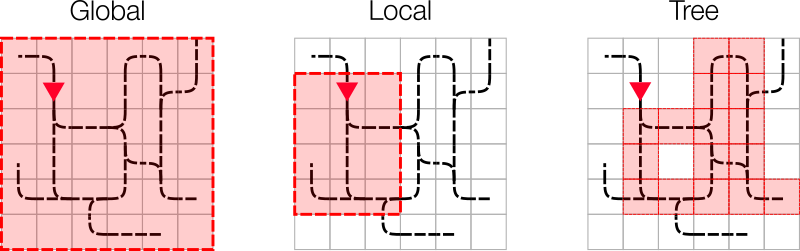
\includegraphics[width=0.5\textwidth]{res/obs.png}
        \caption{\label{fig:Views}Visual summary of the three provided observation.}
        \end{figure}
    \end{itemize}
    
    \item Rewards:
    
    At each time step, each agent receives a combined reward which consists of a \textbf{local} and a \textbf{global} reward signal.
    Locally, the agent receives $r_l=-1$ for each time step, and $r_l=0$ for each time step after it has reached its target.  The global reward signal $r_g$ is equal to $0$ only if all agents have reached their targets, in the opposite case it is worth $1$.
    Every $i-th$ agent receives:
    \[ r_i(t)= \alpha r_l(t) + \beta r_g(t) \]
    $\alpha$ and $\beta$ are two tuning factors to regulate collaborative behaviour. In the 2021 Flatland challenge the provided values are $\alpha = 1.0$ and $\beta = 1.0$
\end{itemize}

\subsubsection{Malfunctions}

Malfunctions are a complication added to the Flatland problem to simulate delays by stopping agents at random times for random duration. 
This random value is implemented using a Poisson process. 
Train that malfunction can’t move for a random, but known, number of steps and they block the trains following them.

\section{Solution}

\subsection{Deep Q-Networks (DQN)}

DQN \cite{atari} are the tool used for applying Deep Q-Learning. The main idea is to unify Q-Learning and Deep Learning for dealing with complex environments. 
To achieve that a neural network is used as a predictor of the $Q(s, a)$ function.

To achieve an exploration behaviour a $\epsilon$ parameter with a decaying factor is used as a probability of performing random actions. The more time passes (resulting in the network being trained more) the lower the probability of exploring.

By performing training on subsequent states the dataset wouldn't be ideally distributed. To deal with those issues, training is done over a large buffer of the past experiences used to sample training data from it. This technique is called \textbf{replay buffer}. The simplest implementation of it keeps a fixed size, having new data added to the end of the buffer for every agent step such that it pushes the oldest experience out of it. 

The main algorithm's steps are:
\begin{enumerate}
    \item Initialize $Q(s,a)$ with some initial approximation
    \item By interacting with the environment, obtain the tuple \textit{(s,a,r,s')}
    \item Calculate loss: $\mathcal{L} =(Q(s,a)-r)^2$ if the episode has ended, or $\mathcal{L} =(Q(s,a)-(r+\gamma max_{a' \in A} Q_{s',a'}))^2$ otherwise
    \item Update $Q(s,a)$ using the \textbf{stochastic gradient descent (SGD)} algorithm, by minimizing the loss with respect to the model parameters.
    \item Repeat from step 2 until converged.
\end{enumerate}

First of all, we need to interact with the environment somehow, to receive data to train on. In simple environments, acting randomly could be considered, but in a more difficult environment the probability of achieving the goal by acting randomly is extremely small. The alternative is to use Q-function approximation, if our representation of Q is good, then the experience that agent gets from the environment will show relevant data to train on. However, if the approximation is not perfect, the agent can be stuck with bad actions for some states without ever trying to behave differently. This problem is also called \textit{Exploration versus Exploitation} dilemma. On one hand, agent needs to explore the environment to build a complete picture of transitions and action outcomes by performing random actions. On the other hand, interaction with the environment should be efficient: we shouldn't waste time by randomly trying actions that were already tried and have learned outcomes for. 
So random behaviour is better at the beginning of the training when our Q approximation is bad, since it gives more uniformly distributed information about the environment states. As the training goes on, random behaviour becomes inefficient, therefore we want to go back to our Q approximation to decide how to act.
A method that performs such mix of behaviours is known as \textbf{epsilon-greedy method}, which means switching between random policy and Q policy using the probability hyperparameter $\epsilon$. By varying $\epsilon$, we tune the ratio of random actions. It is usual practice to start with $\epsilon = 1$ (purely random) and slowly decrease it to some small value (5\% or 2\%).

The core of the Q-learning procedure is borrowed from supervised learning. Indeed, we are trying to approximate a complex, nonlinear function \textit{Q(s,a)} with a Neural Network. To do this, we must compute targets for this function using the Bellman equation and then pretend to have a supervised learning problem at hand. That's not a problem, but one of the fundamental requirements for SGD optimization is that the training data is independent and identically distributed (i.i.d.). The data used for SGD update doesn't fulfill the following criteria:
\begin{itemize}
    \item Our samples are not independent. Even if a large batch of data samples is available, they will all be very close to each other, as they belong to the same episode.
    \item Distribution of our training data won't be identical to samples provided by the optimal policy that must be learned. The data we'll have are results from some other policy (custom policy, random policy or both in case of epsilon-greedy method). 
\end{itemize}

To deal with those issues, it's usually used a large buffer of the past experience and sample training data from it, instead of using last experience. This technique is called \textbf{replay buffer}. The simplest implementation of it is of fixed size, where new data will be added to the end of the buffer such that it pushes the oldest experience out of it. There exist lots of different implementation of the buffer with different policies of storing data. 

The DQN algorithm consists of the following main steps:
\begin{enumerate}
    \item Initialize the parameters for $Q(s,a)$ and $\hat{Q}(s,a)$ with random weights, $\epsilon \leftarrow 1.0$, and empty the replay buffer.
    \item With probability $\epsilon$, select a random action, \textit{a}, otherwise, $a=argmax_aQ(s,a)$.
    \item Execute action \textit{a} in an emulator and observe the reward, \textit{r}, and the next state, \textit{s'}.
    \item Store transition \textit{(s,a,r,s')} in the replay buffer.
    \item Sample a random mini-batch of transitions from the replay buffer.
    \item For every transition in the buffer, calculate target $y=r$ if the episode has ended at this step, or $y=r+\gamma max_{a' \in A} \hat{Q}(s',a')$ otherwise.
    \item Calculate loss: $\mathcal{L}=(Q(s,a) - y)^2$
    \item Update $Q(s,a)$ using the SGD algorithm by minimizing the loss with respect to the model parameters.
    \item Every \textit{N} steps, copy weights from \textit{Q} to $\hat{Q}$.
    \item Repeat from step 2 until converged.
    \end{enumerate}

\begin{figure}[H]
        \centerline{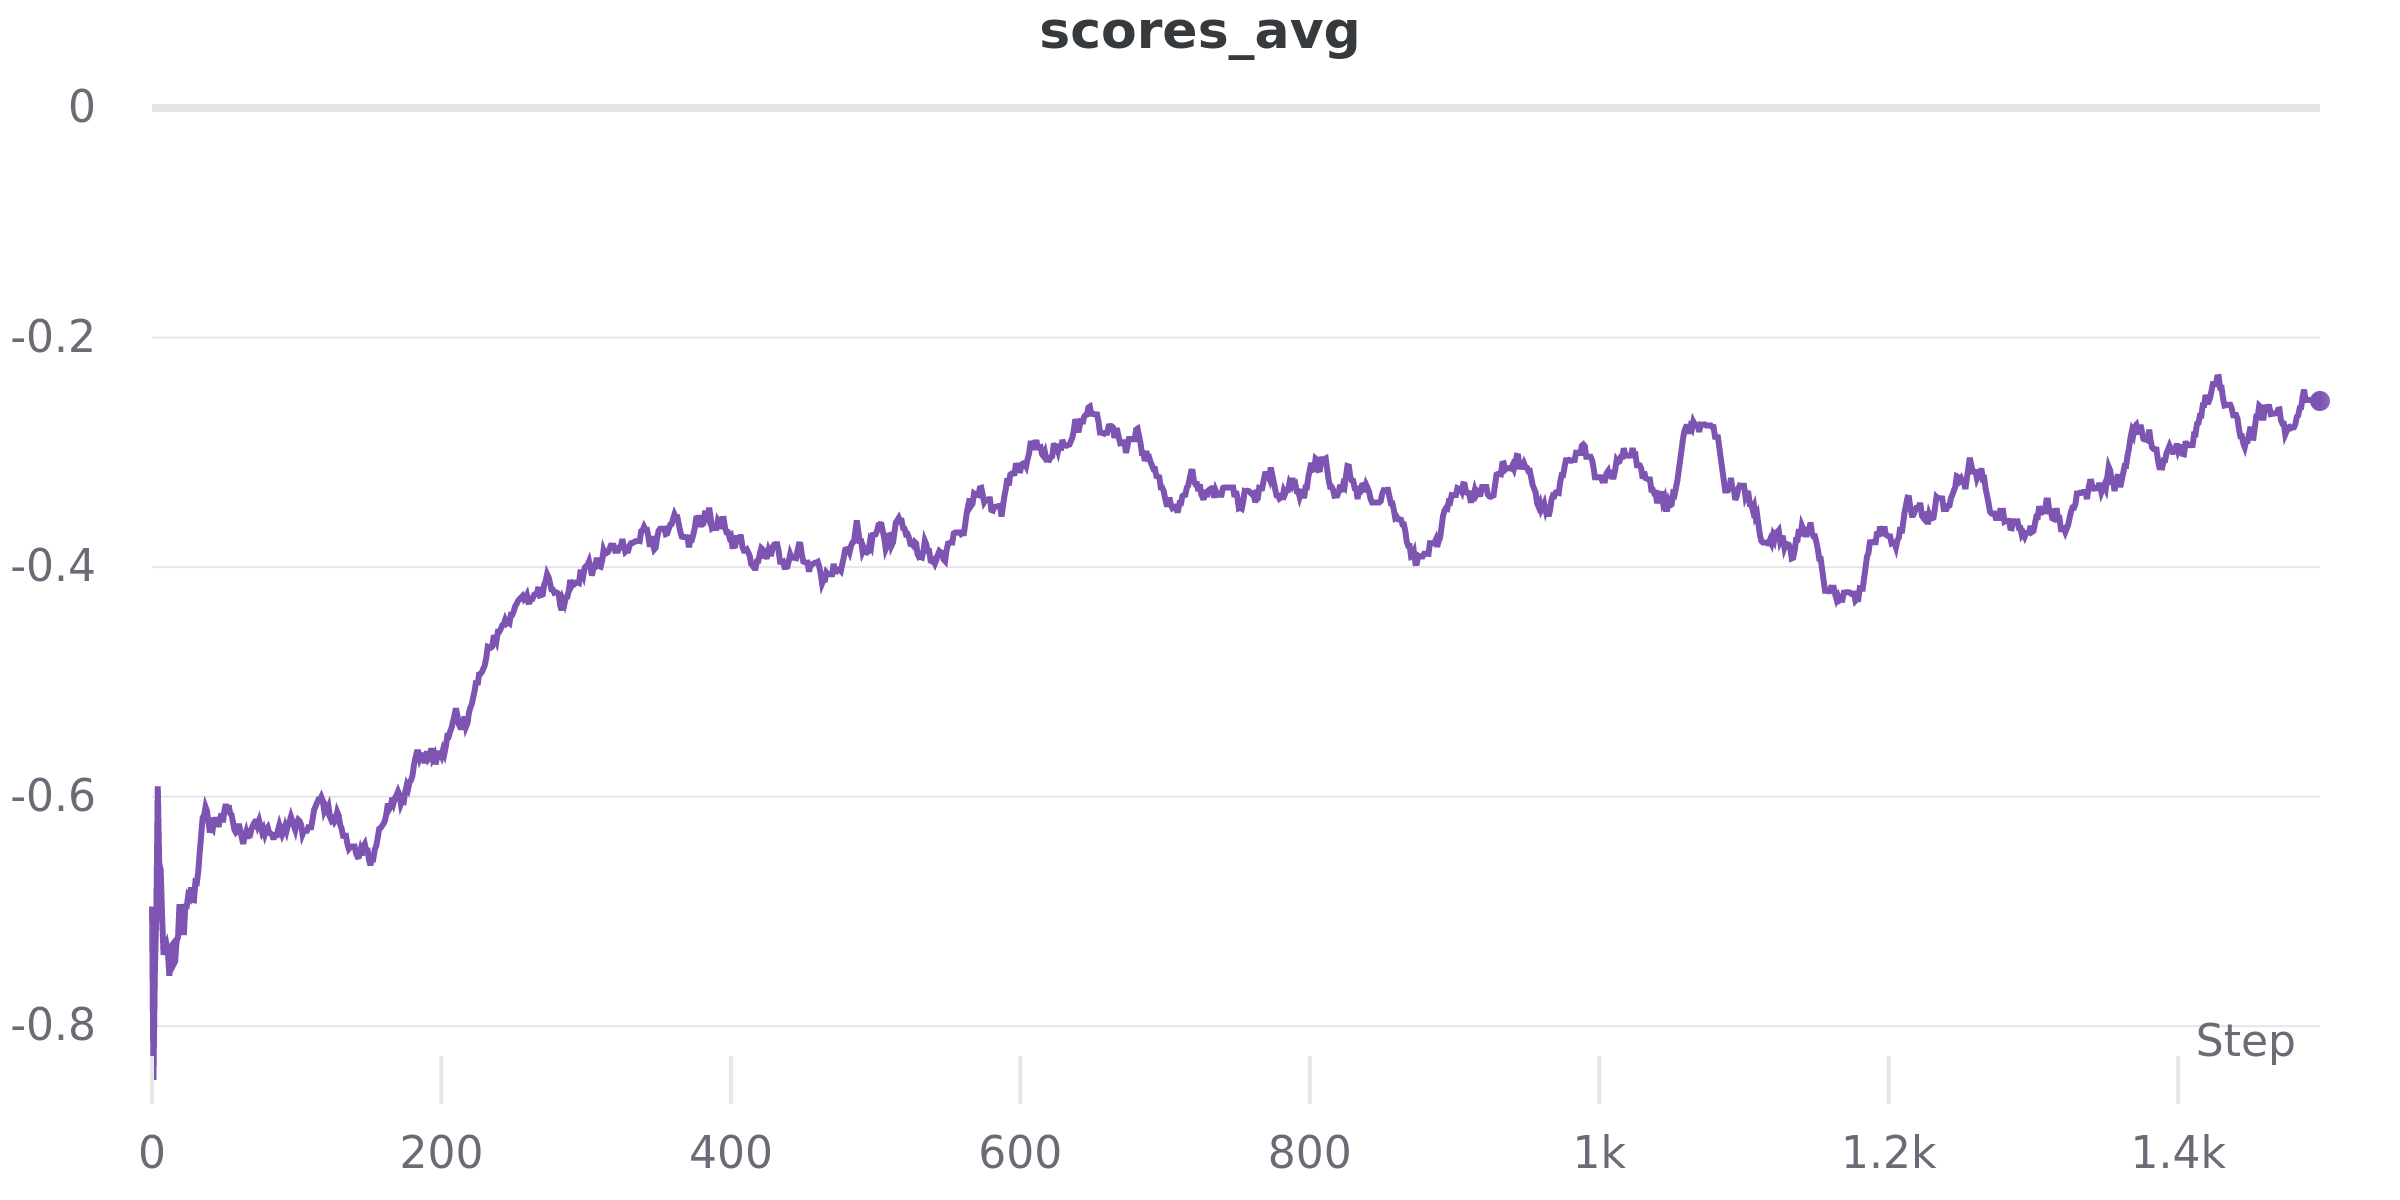
\includegraphics[scale=.2]{res/charts/vanilla_scores.png}}
        \caption{Scores}
\end{figure}

\begin{figure}[H]
        \centerline{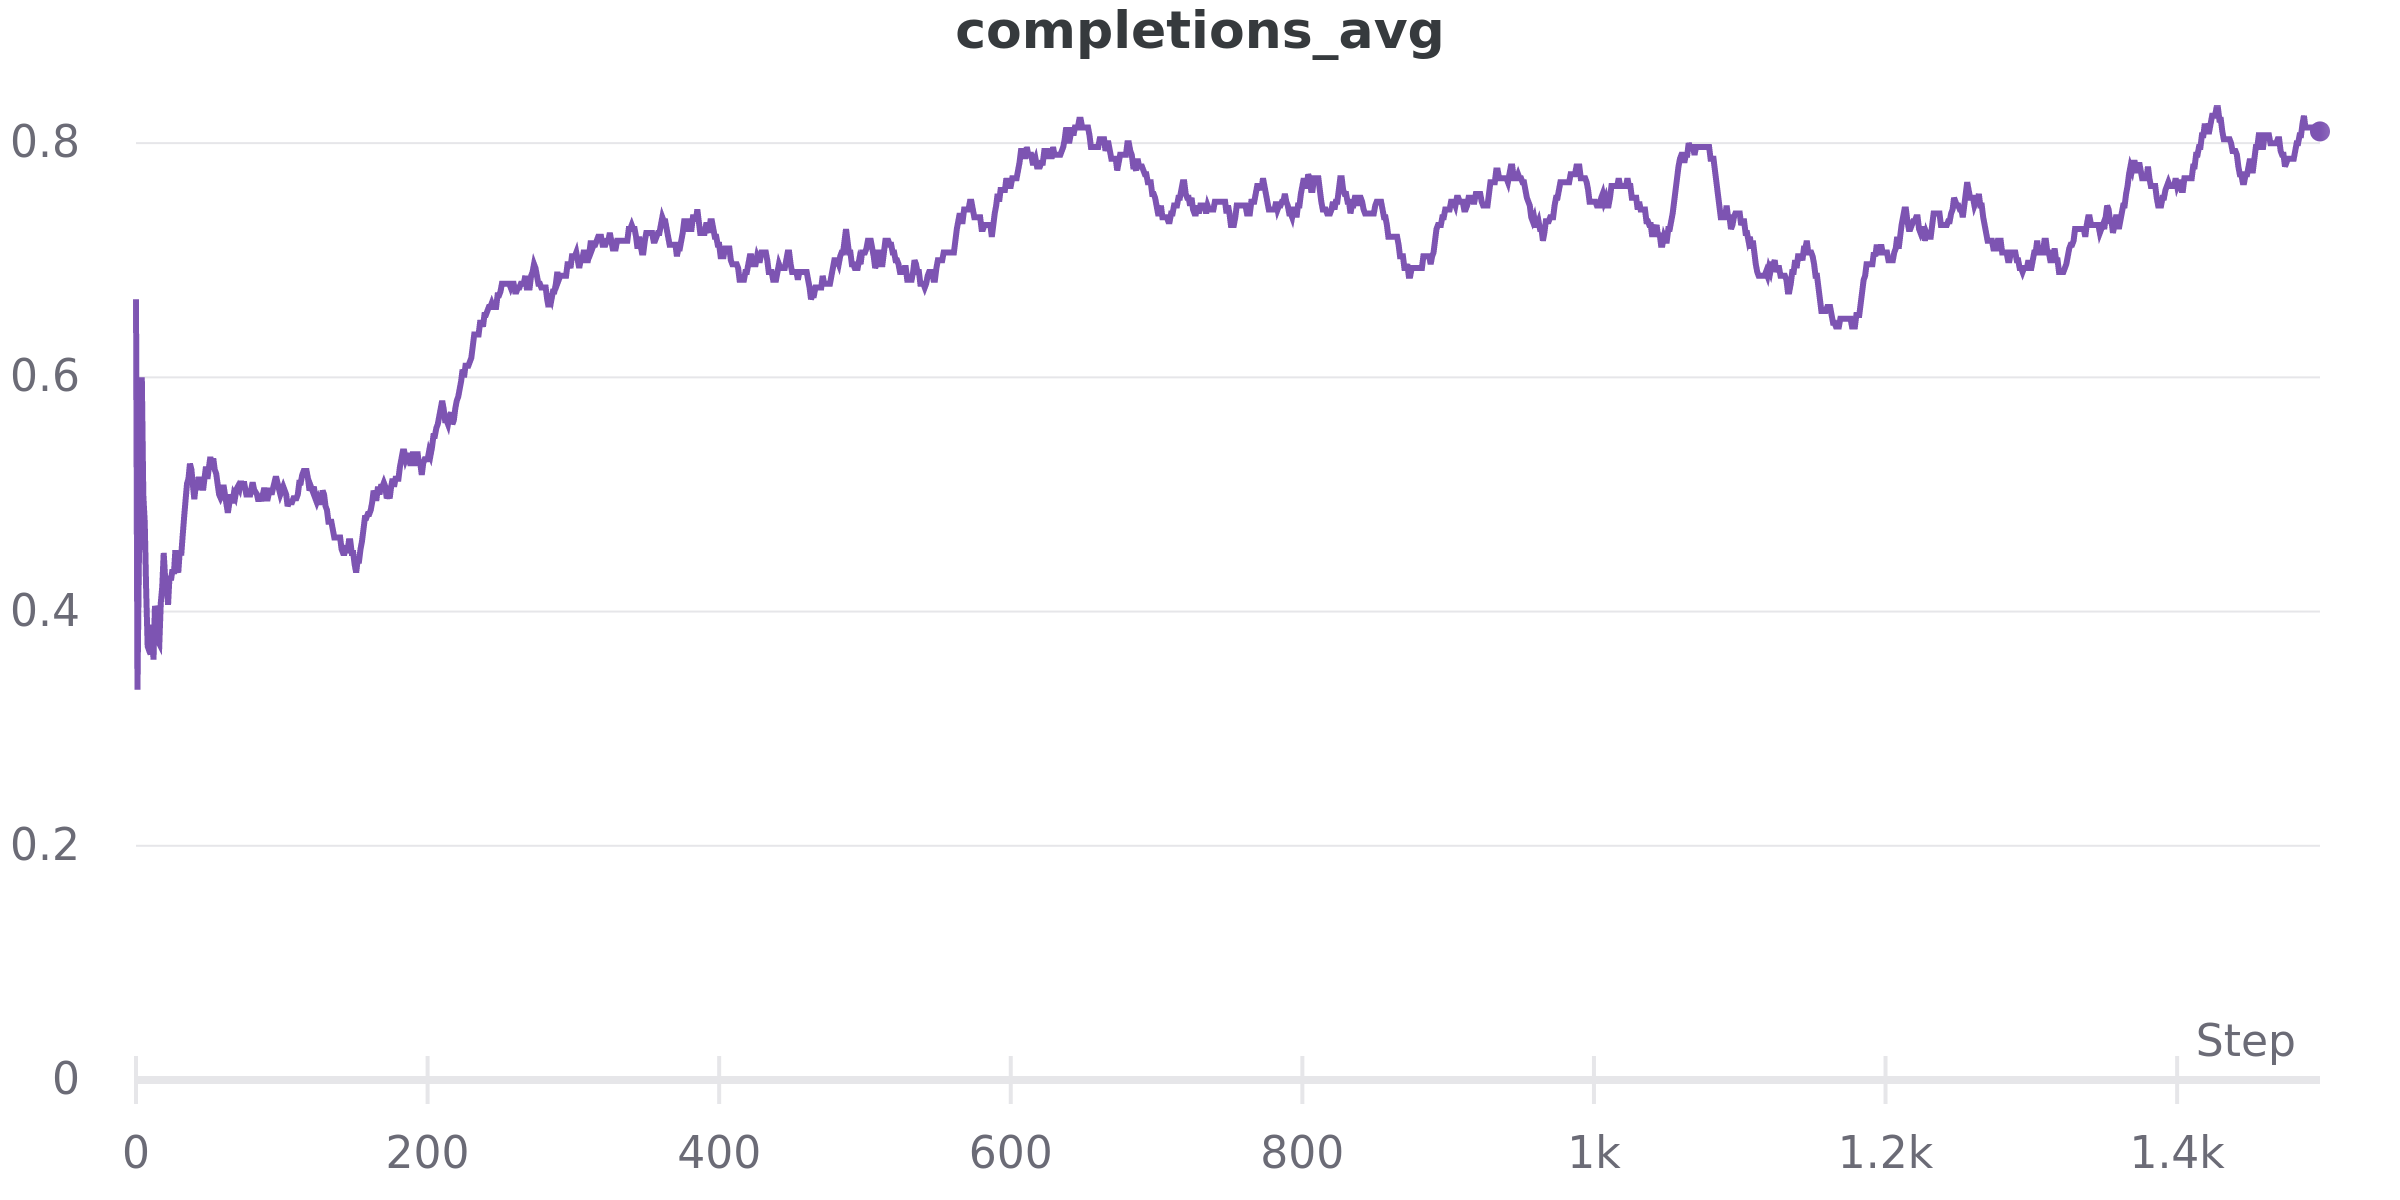
\includegraphics[scale=.2]{res/charts/vanilla_completions.png}}
        \caption{Completions}
\end{figure}

\subsubsection{Double DQN}
DeepMind researches demonstrated that the basic DQN tends to overstimate Q-values (due to the max operation in Bellman equation) \cite{double-dqn}, which could lead to suboptimal policies. Therefore, they tried to update the Bellman equation.
In basic DQN, our target value for Q was:
\[ Q(s_t,a_t)= r_t+\gamma max_a Q'(s_{t+1},a)\]

Where $Q'(s_{t+1},a)$ was Q-values calculated using target network, so we update with the trained network every n steps.
Without going through details, they proposed choosing actions for the next state using the trained network, but taking values of Q from the target network.

\[ Q(s_t,a_t)= r_t+\gamma max_a Q'(s_{t+1},argmax_a Q(s_{t+1},a))\]

This little tweak is proved to fix the overstimation completely and is called \textbf{Double DQN}.

TODO Io farei così

Double DQN \cite{double-dqn} is a simple tweak to the basic method consisting in exploiting the usage of a second neural network (called \textit{target network}), which TODO (dire cosa fa la target). This is an attempt to overcome the Q-values overestimation problem which afflicts vanilla DQN.


\begin{figure}[H]
        \centerline{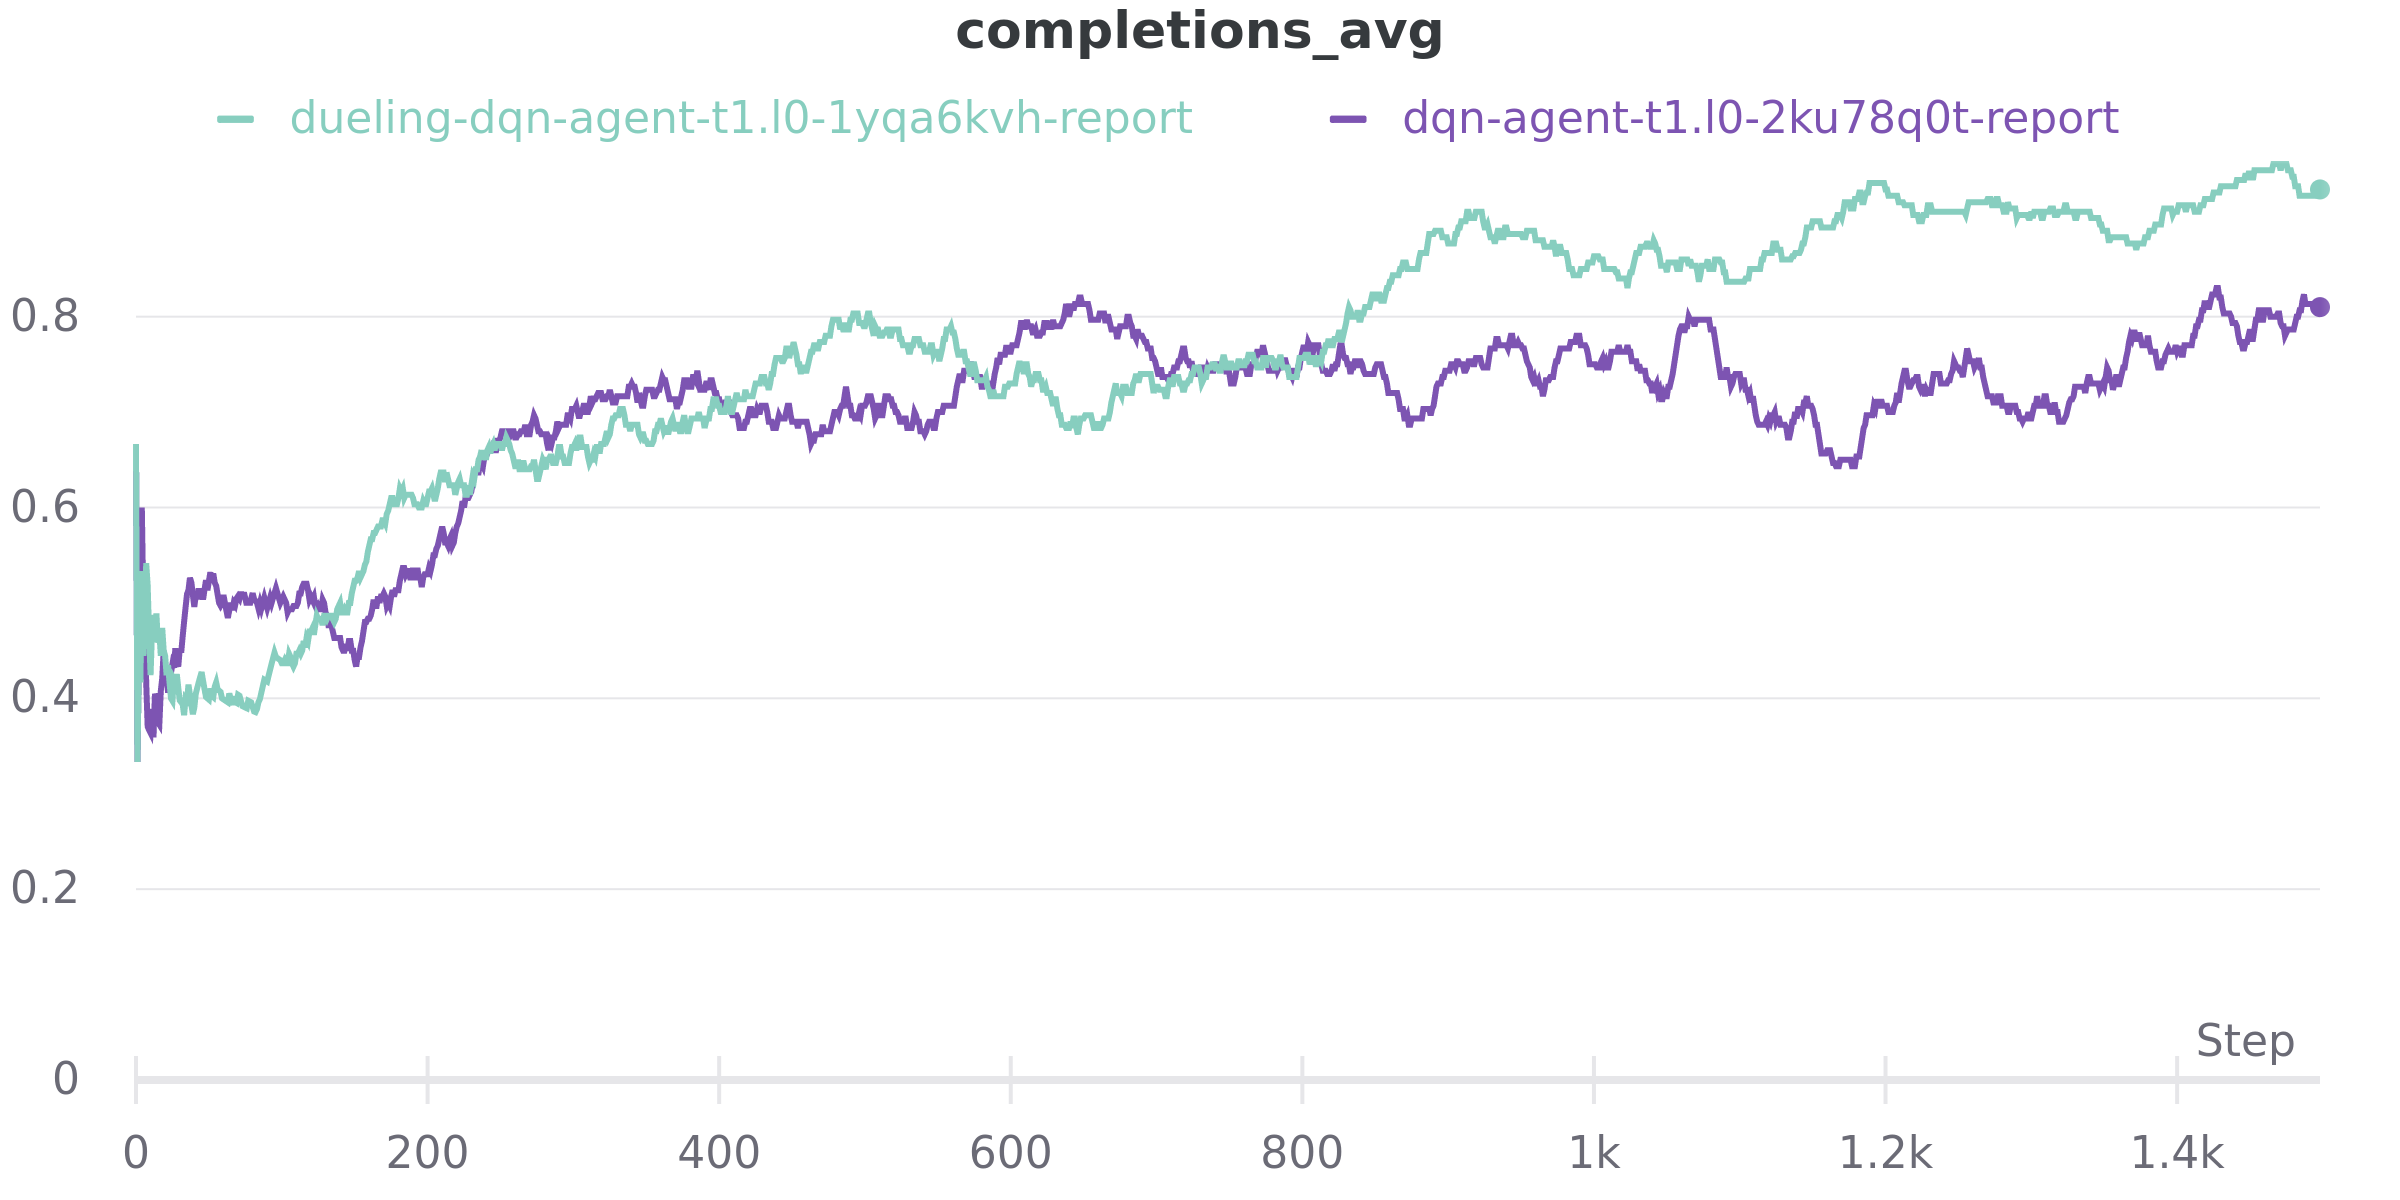
\includegraphics[scale=.2]{res/charts/double_scores.png}}
        \caption{Scores}
\end{figure}

\begin{figure}[H]
        \centerline{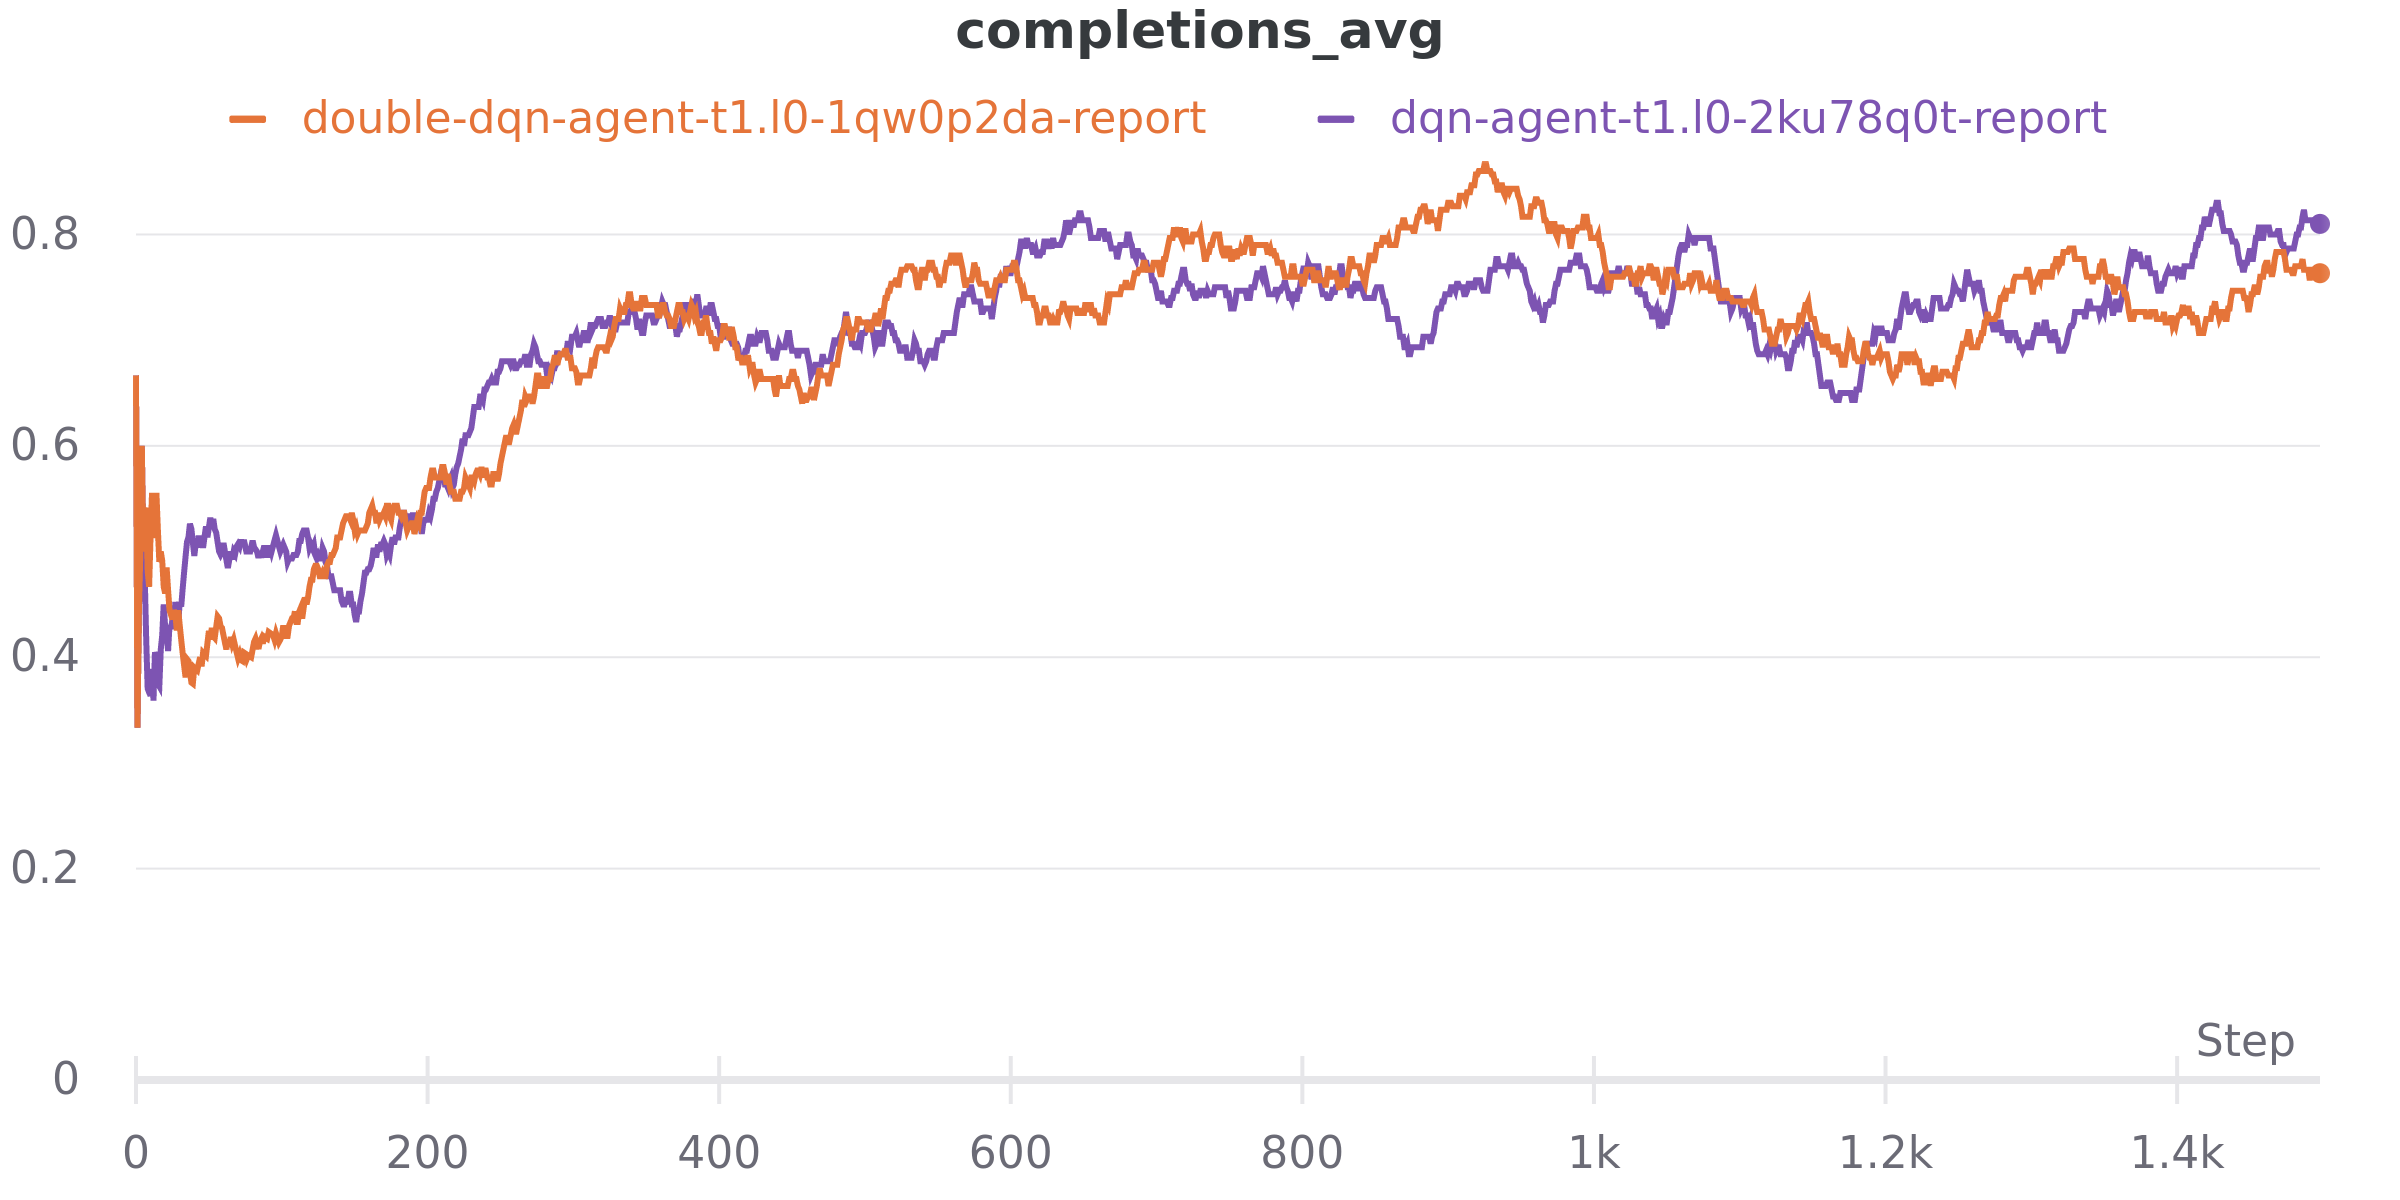
\includegraphics[scale=.2]{res/charts/double_completions.png}}
        \caption{Completions}
\end{figure}

TODO Ao ce sta anche il soft update che è molto figo.

\begin{figure}[H]
        \centerline{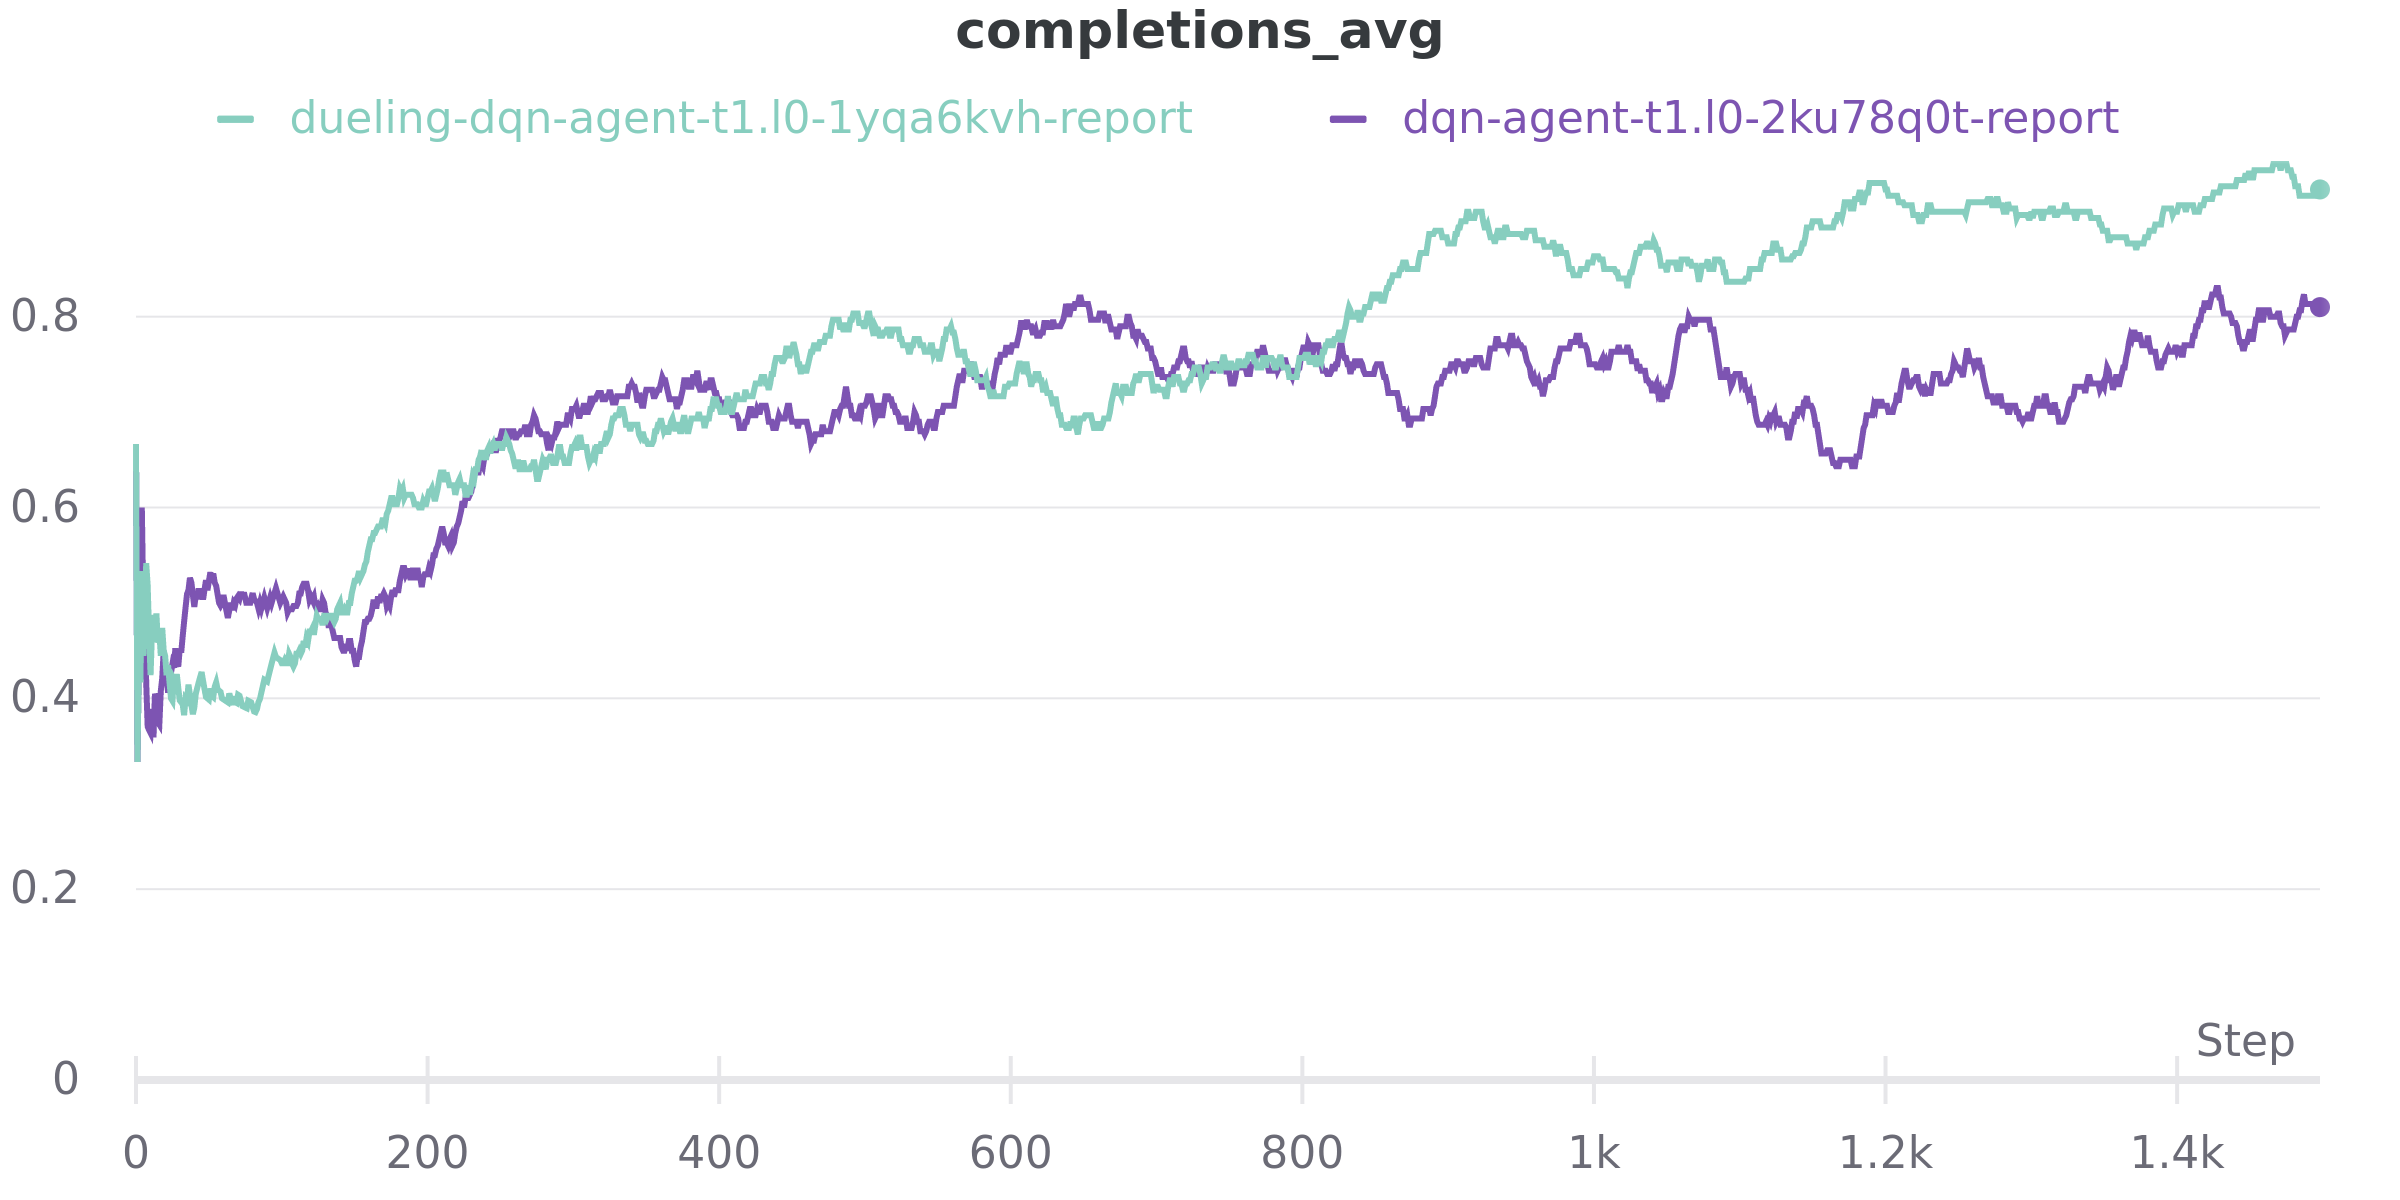
\includegraphics[scale=.2]{res/charts/double_scores.png}}
        \caption{Scores}
\end{figure}

\begin{figure}[H]
        \centerline{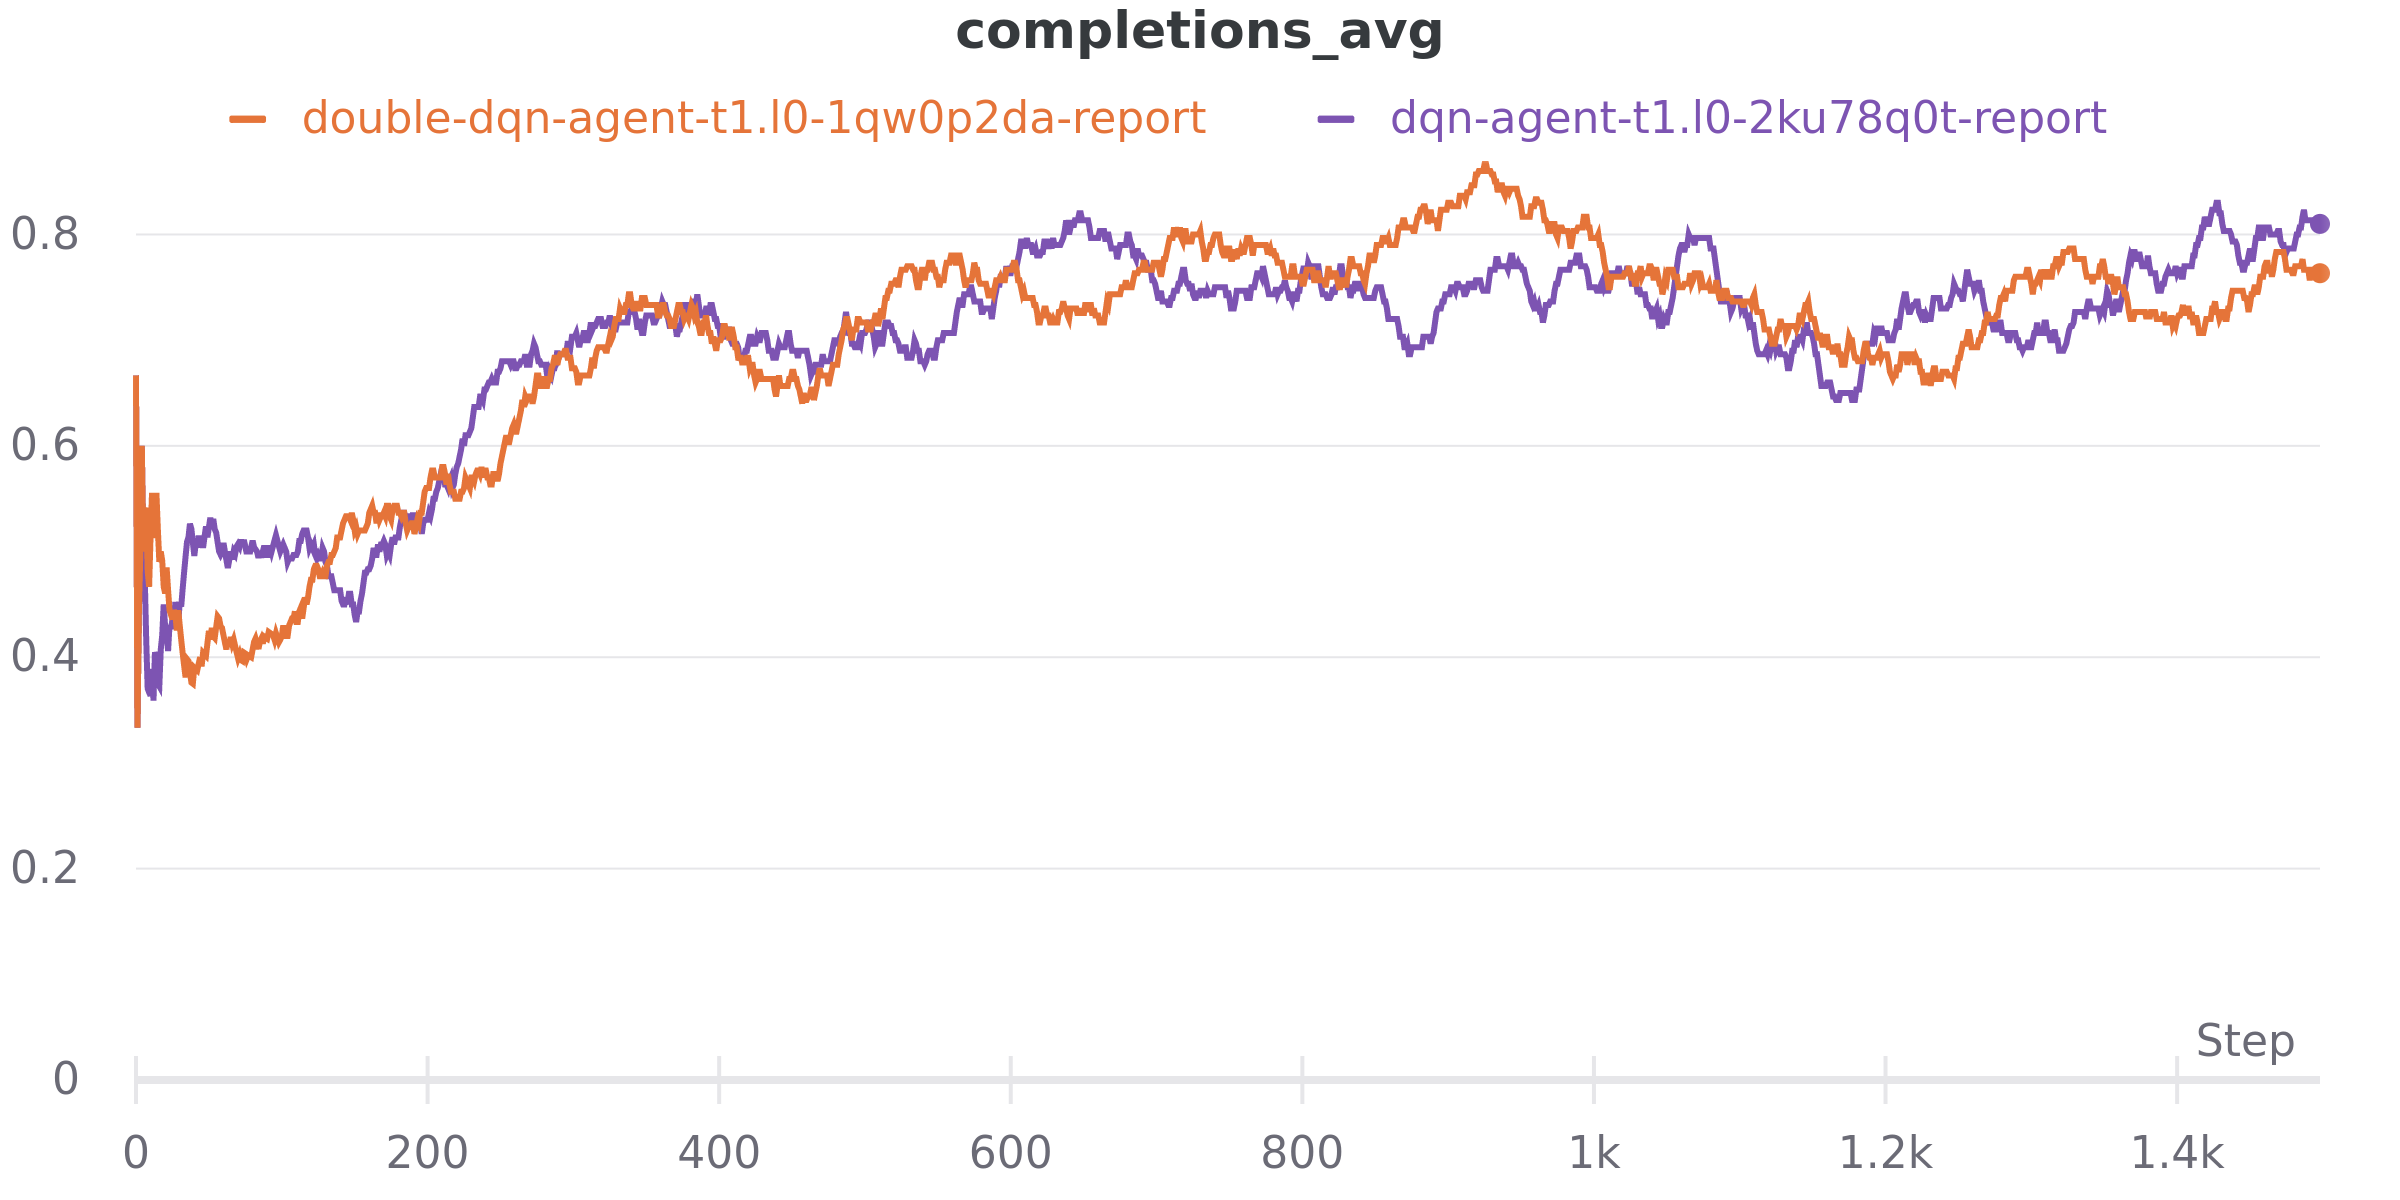
\includegraphics[scale=.2]{res/charts/double_completions.png}}
        \caption{Completions}
\end{figure}

\subsubsection{Dueling DQN}
Q-values, $Q(s,a)$, that our network is trying to approximate can be divided into quantities: the value of the state, $V(s)$, and the advantage of actions in this state, $A(s,a)$. The advantage is supposed to bridge the gap from $A(s)$ to $Q(s,a)$, by definition, $Q(s,a)=V(s) + A(s,a)$. In other words, the advantage, $A(s,a)$ is just a delta, saying how much extra reward some particular action from the state brings us. The dueling DQN explicitly separate the value of the state and the advantage into different network's architecture, which brought better training stability, faster convergence. The classic DQN network takes features from the layer and, using dense layers, transforms them into a vector of Q-values, one for each action. Instead, dueling DQN takes features and process them using two independent paths, one path responsible for $V(s)$ prediction (a single number) and the other path predicts individual advantage values, having the same dimension as Q-values in the classic case \cite{dueling-dqn}. After that, $V(s)$ is added to every value of $A(s,a)$ to obtain $Q(s,a)$. 
This constraint could be enforced in different ways, via the loss function or directly by affecting the Q expression subtracting the mean value of the advantage.
\[ Q(s,a)= V(s) + A(s,a) - \frac{1}{N} \sum_k A(s,k) \]

\begin{figure}[H]
        \centerline{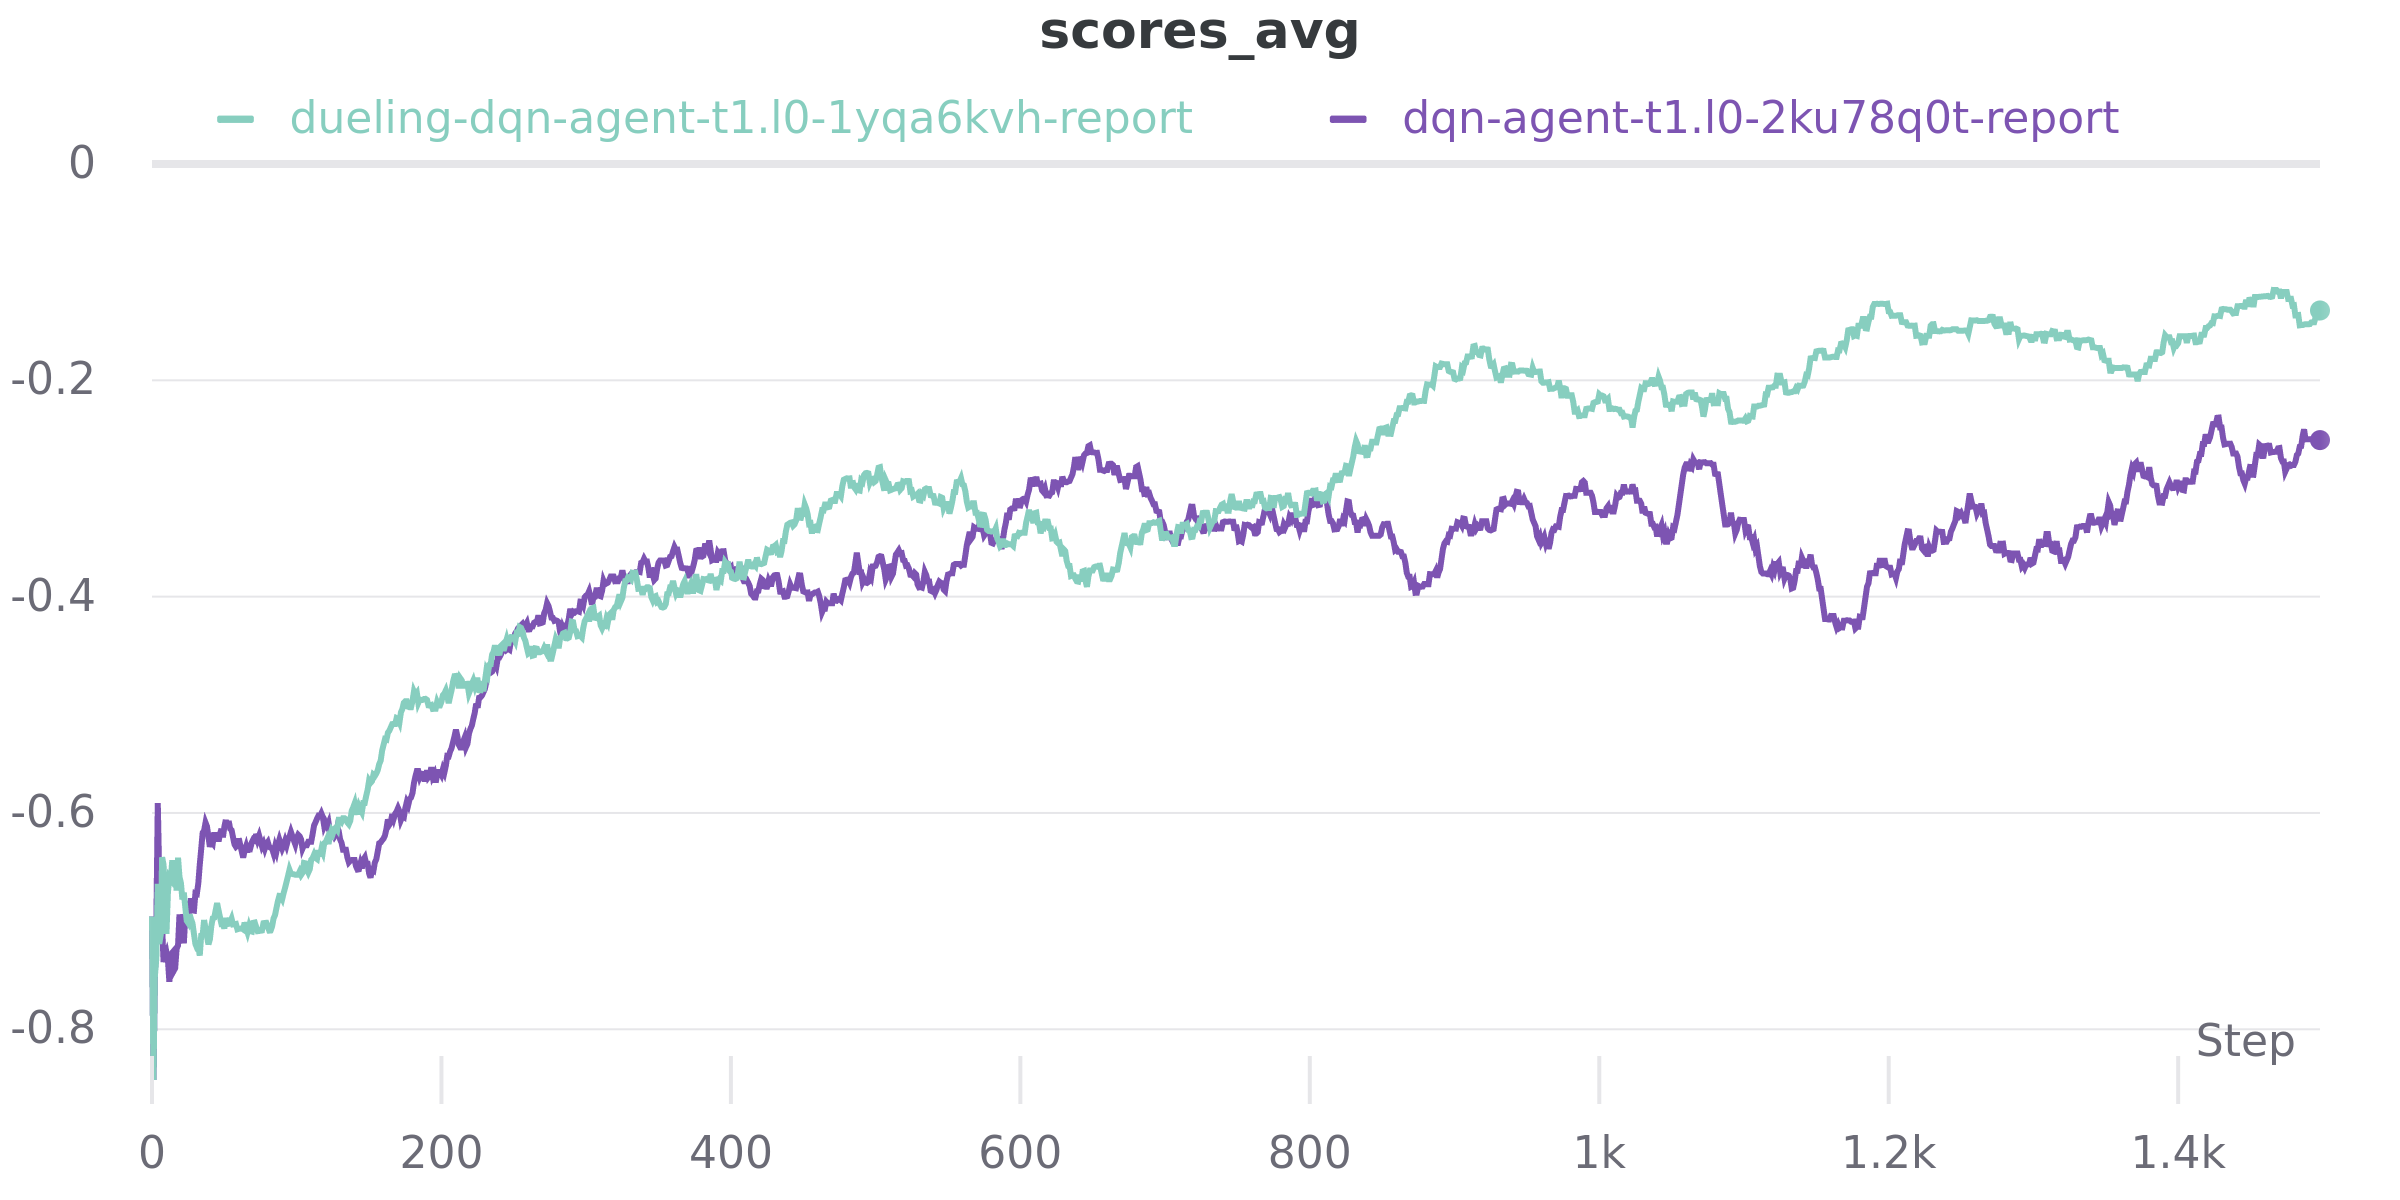
\includegraphics[scale=.2]{res/charts/dueling_scores.png}}
        \caption{Scores}
\end{figure}

\begin{figure}[H]
        \centerline{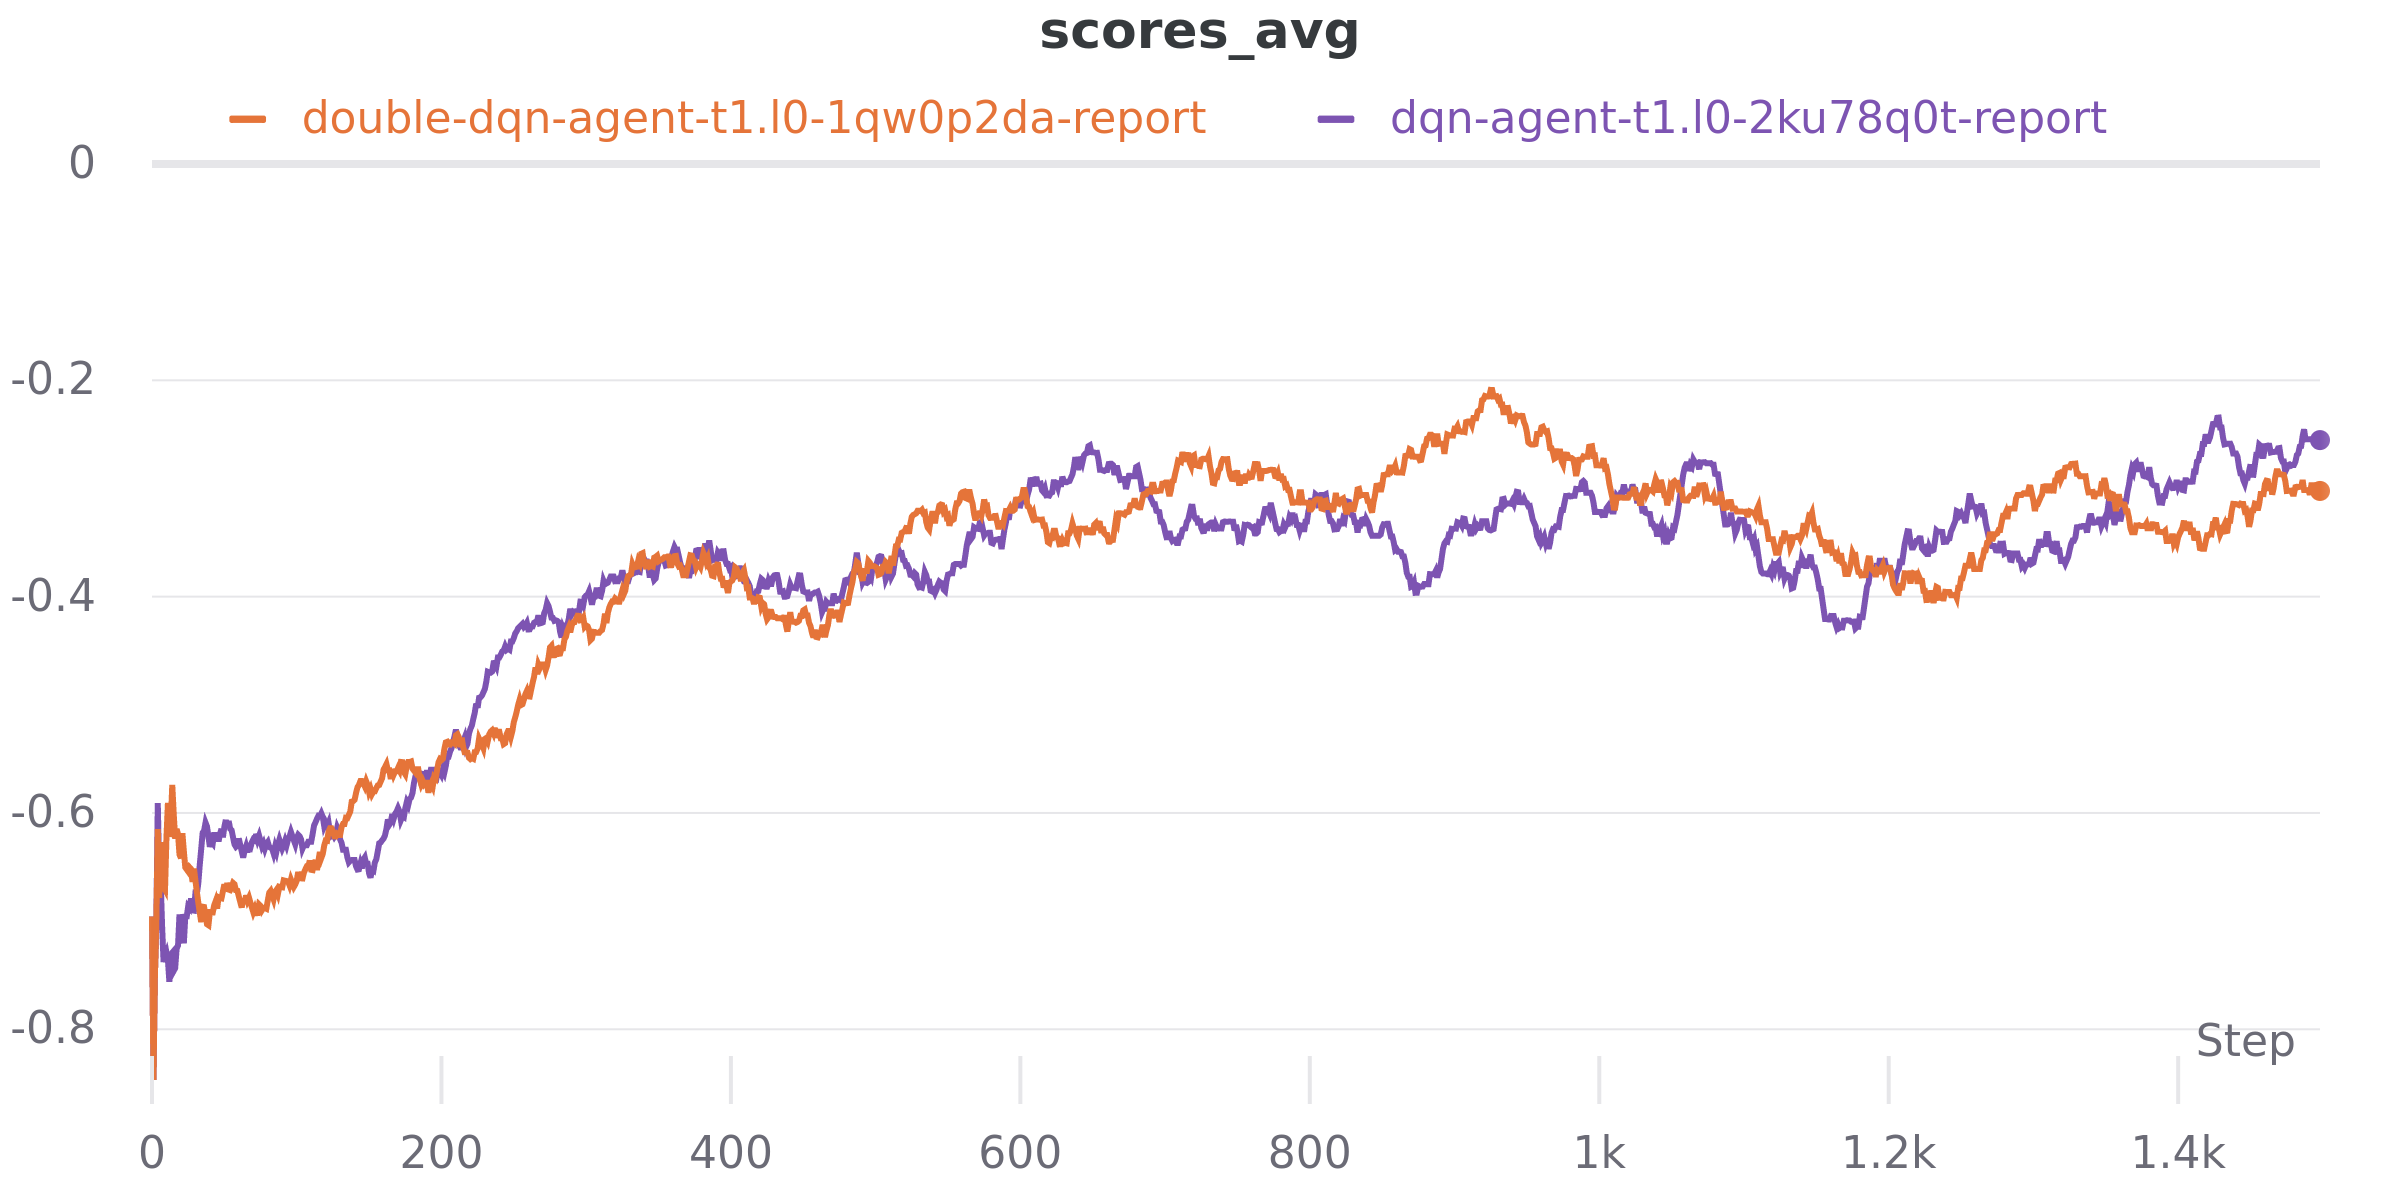
\includegraphics[scale=.2]{res/charts/dueling_completions.png}}
        \caption{Completions}
\end{figure}


\subsubsection{Noisy Networks}
We've talked about the exploration environment via the \textit{epsilon-greedy method}. This process works well for simple environments with short episodes. In Noisy Network's paper \cite{noisy-dqn} the author proposed a simple but well working solution: add noise to the weights of fully connected layers and adjust the parameters of this noise during training using back propagation.  

The authors proposed two ways of adding the noise, both of them work according to their experiments,
but they have different computational overheads:
\begin{enumerate}
    \item \underline{Independent Gaussian noise}: for every weight in a fully connected layer, we have a random
    value that we draw from the normal distribution. Parameters of the noise, $\mu$ and $\sigma$, are stored
    inside the layer and get trained using backpropagation in the same way that we train weights of the
    standard linear layer. The output of such a ``noisy layer" is calculated in the same way as in a linear layer.
    \item \underline{Factorized Gaussian noise}: to minimize the number of random values to be sampled, the
    authors proposed keeping only two random vectors: one with the size of the input and another
    with the size of the output of the layer. Then, a random matrix for the layer is created by
    calculating the outer product of the vectors.
\end{enumerate}

\begin{figure}[H]
        \centerline{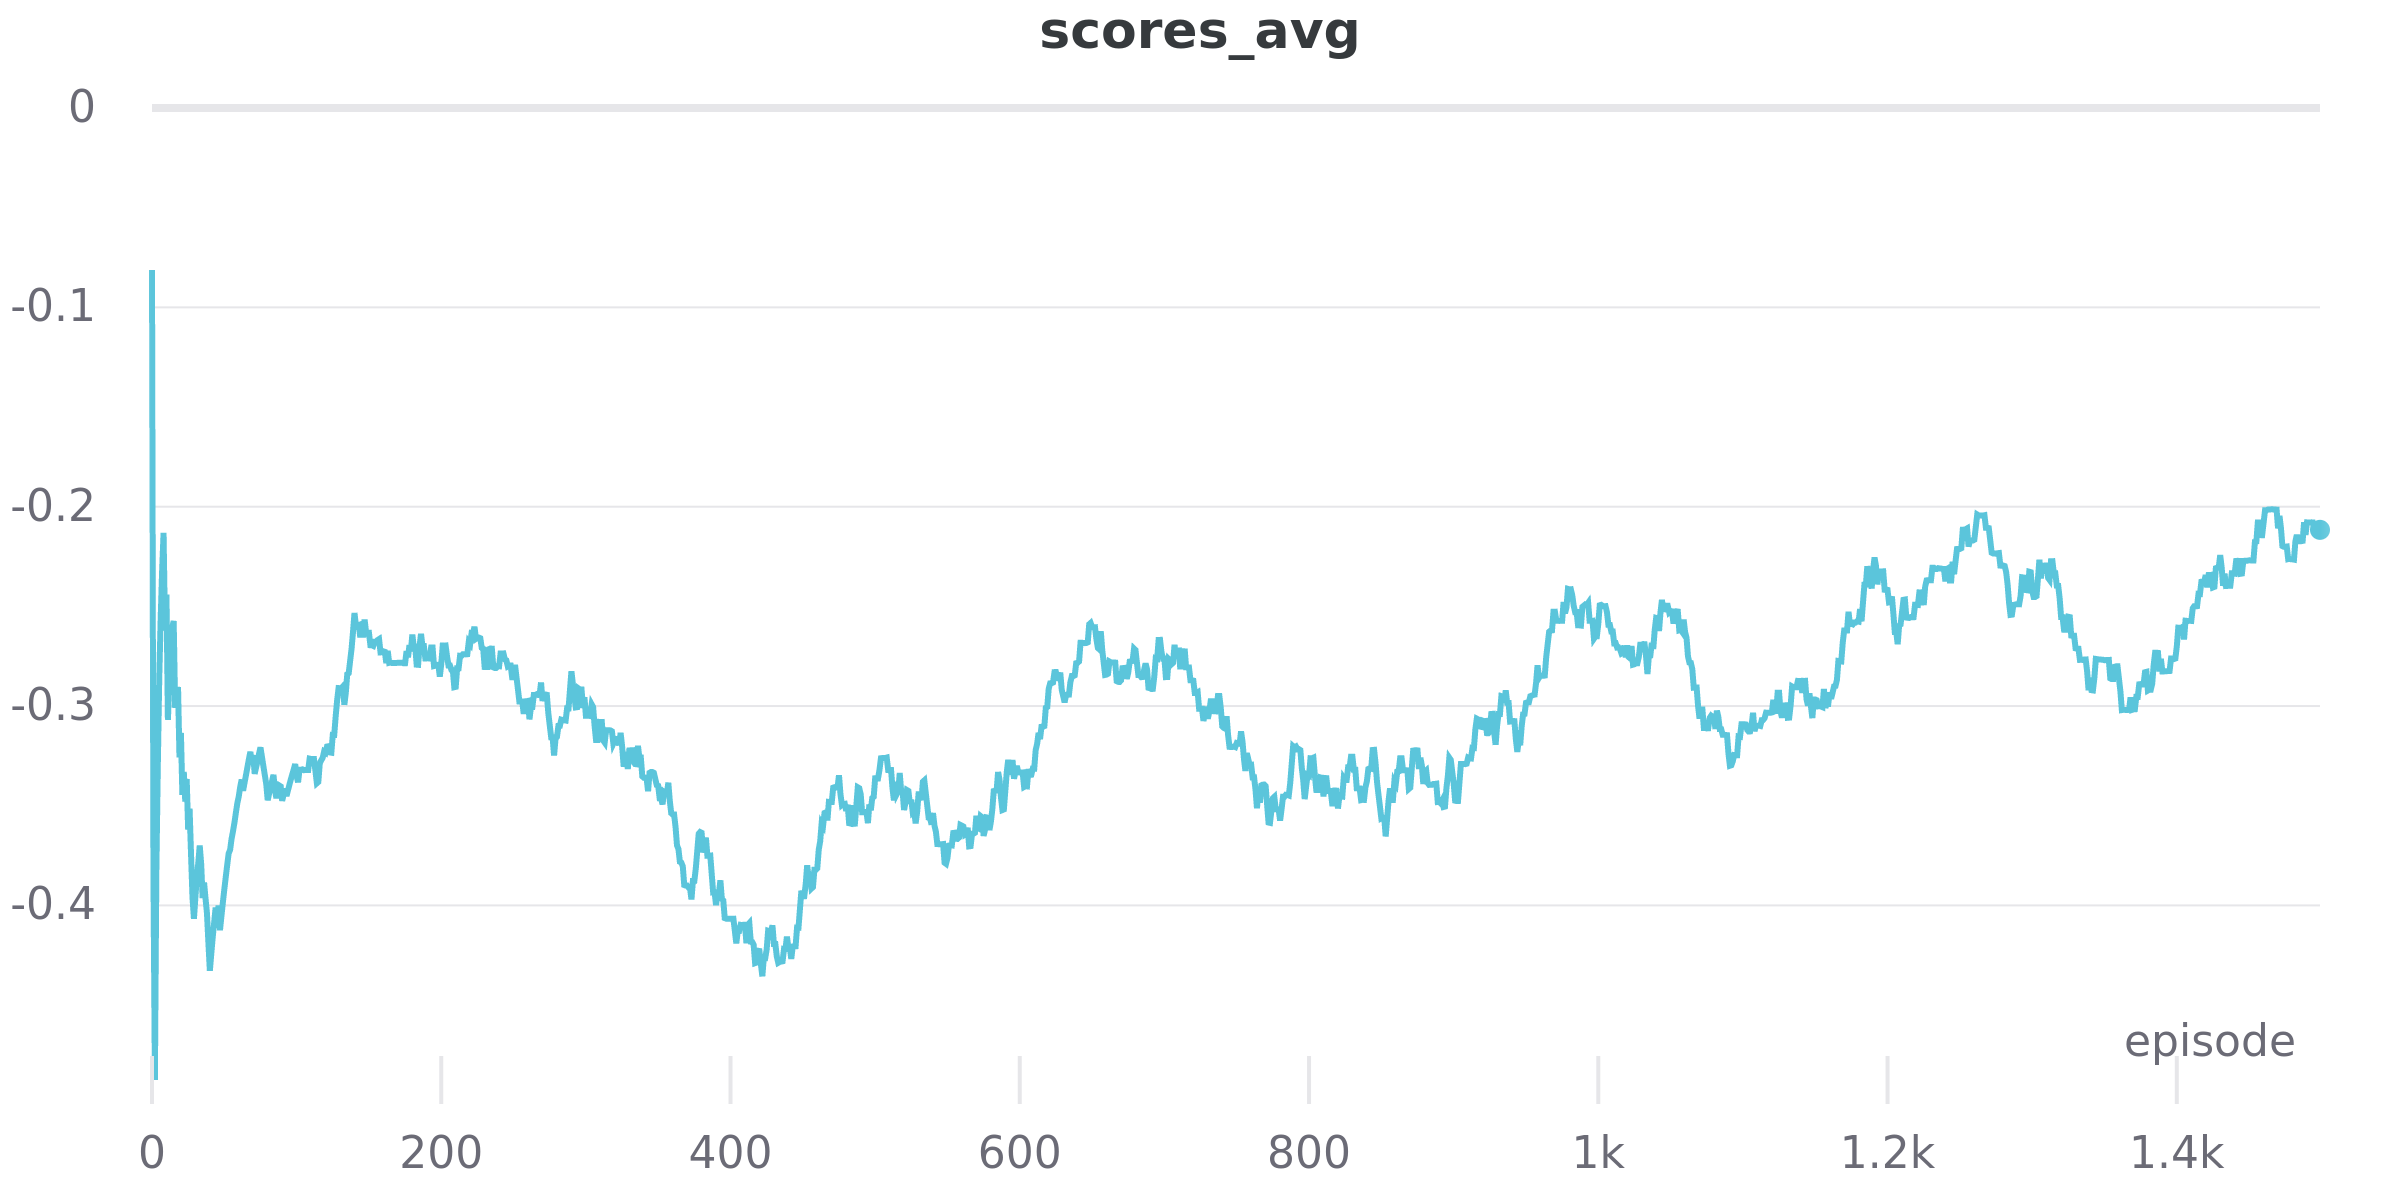
\includegraphics[scale=.2]{res/charts/noisy_scores.png}}
        \caption{Scores}
\end{figure}

\begin{figure}[H]
        \centerline{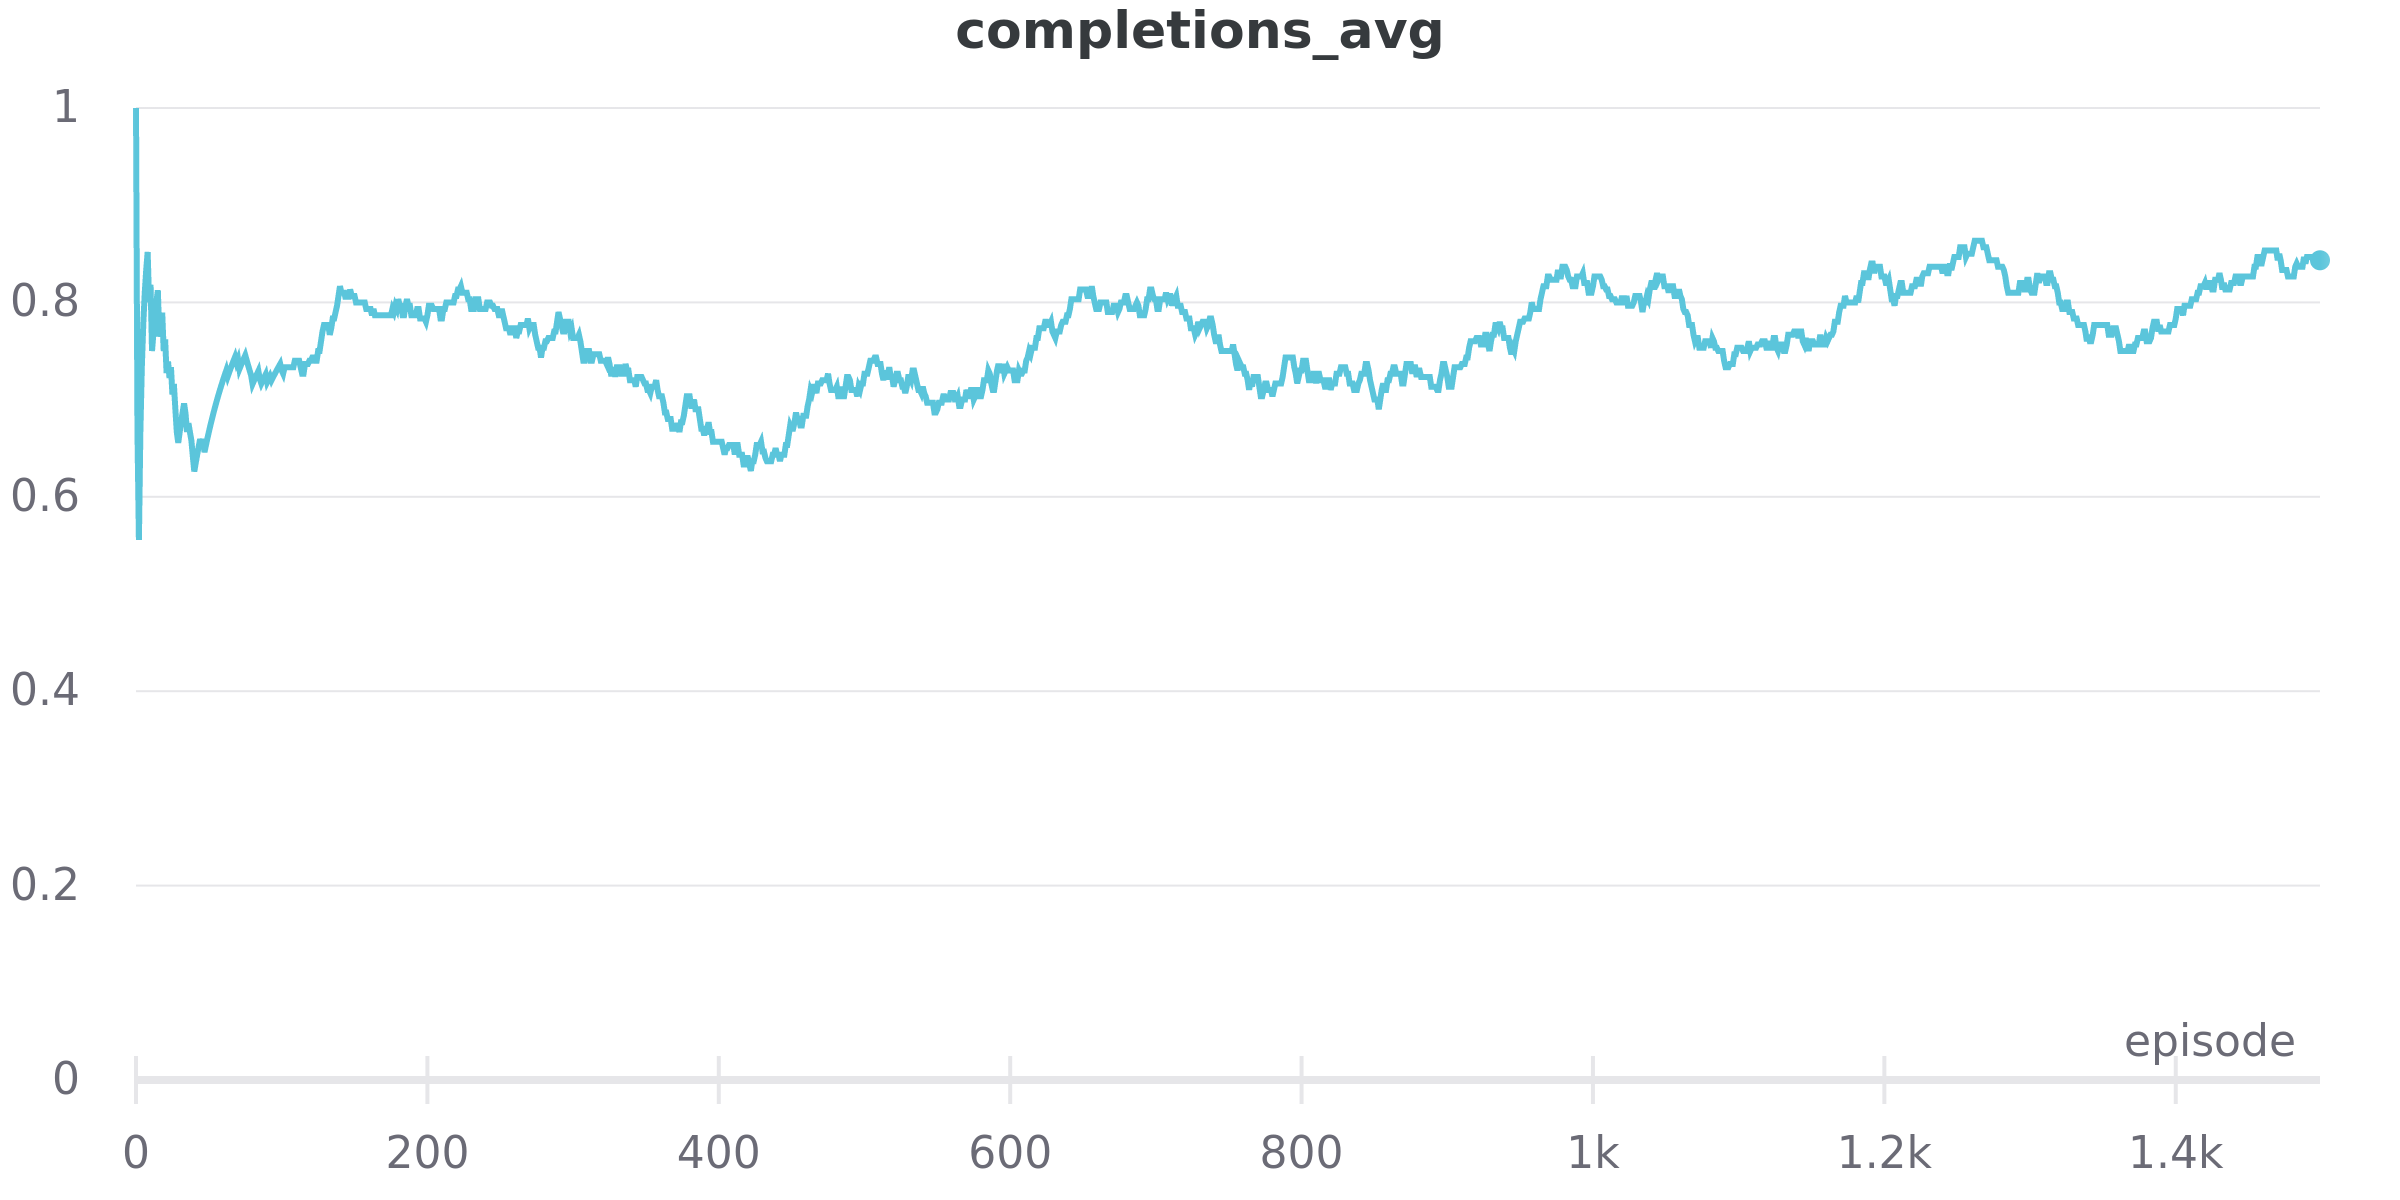
\includegraphics[scale=.2]{res/charts/noisy_completions.png}}
        \caption{Completions}
\end{figure}

\subsubsection{Prioritized Experience Replay}
The classic DQN can be improved in all aspects, also, in how to deal with the experience replay.
Prioritized replay buffer \cite{per} works by assigning priorities to buffer samples, according to training loss and sampling from it proportionally to the priorities. The basic idea of PER is to train on data that ``surprised" the system. The sensitive point, is to maintain balance between training on ``unusual" samples and training on the rest of the buffer.
The priority of every sample in the buffer is:
\[ P(i)= \frac{p^\alpha _i}{\sum_k P^\alpha _k} \]

Where $p_i$ is the priority of the \textit{i-th} sample in the buffer and $\alpha$ is a parameter that expresses the importance we give to the priority. If $\alpha=0$, our sampling will become uniform as in the classic DQN method. Larger values of $\alpha$ put more stress on samples with higher priority. It is general usage to start with $\alpha=0.6$.  
By adjusting the priorities for the samples, bias is introduced into our data distribution (where we sample some transition much more frequently than others) that need to be compensated for SGD to work. To get this result, the priority value is modified as follows:

\[w_i=(N \cdot  P(i))^\beta ,\quad \beta \in [0,1]\]

If $\beta = 1$, the bias introduced by the sampling is fully compensated. Anyway, the general usage it to start with a random value between 0 and 1 and slowly increase it to 1 during the training.


\begin{figure}[H]
        \centerline{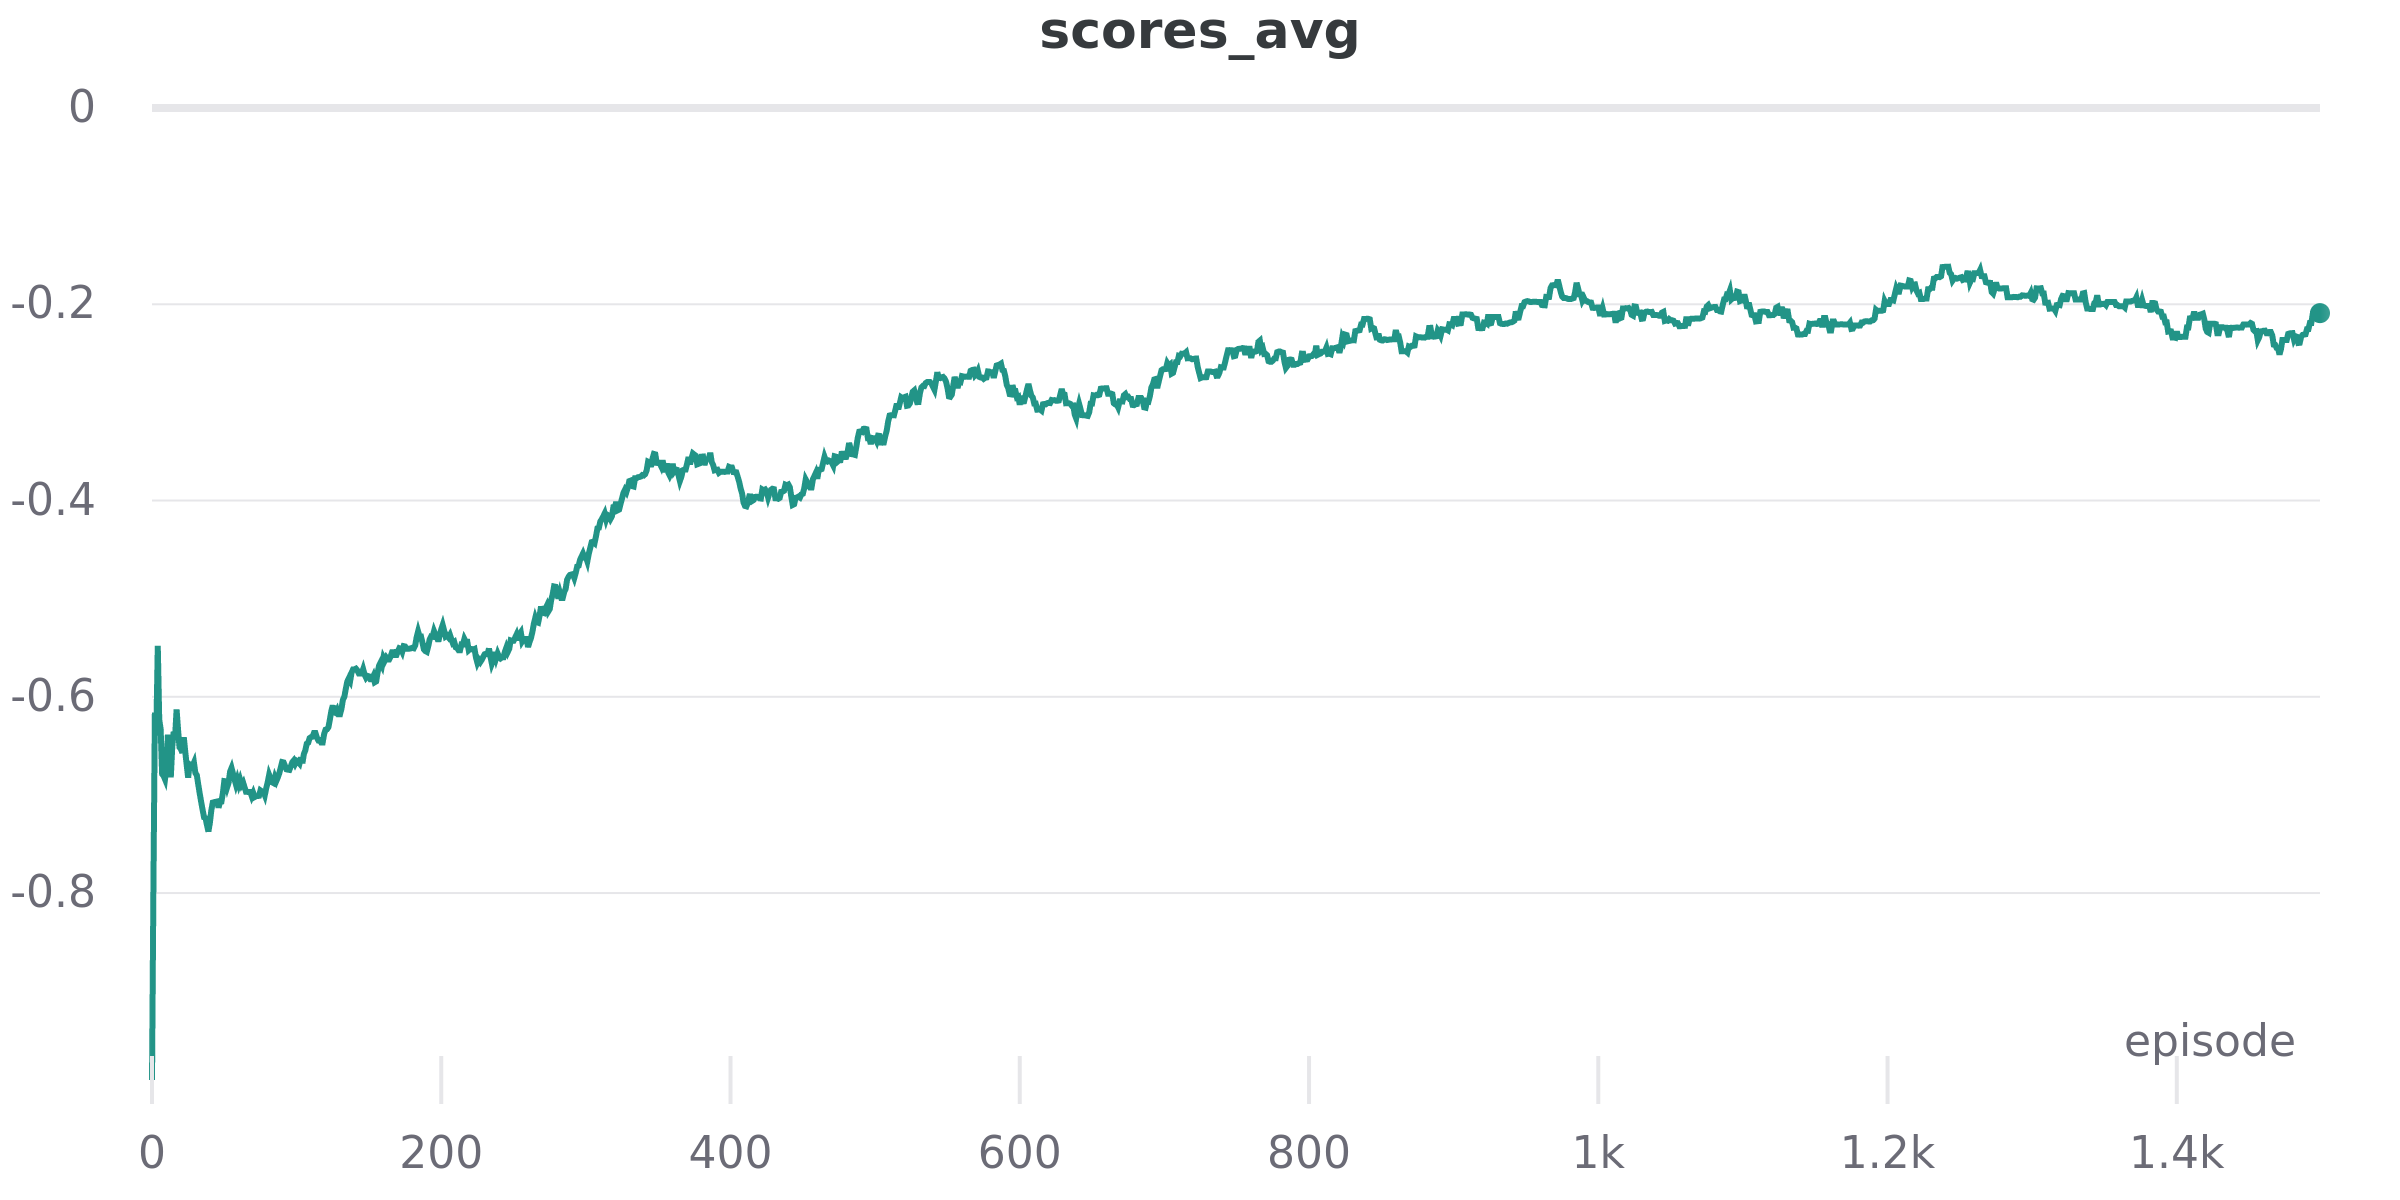
\includegraphics[scale=.2]{res/charts/per_scores.png}}
        \caption{Scores}
\end{figure}

\begin{figure}[H]
        \centerline{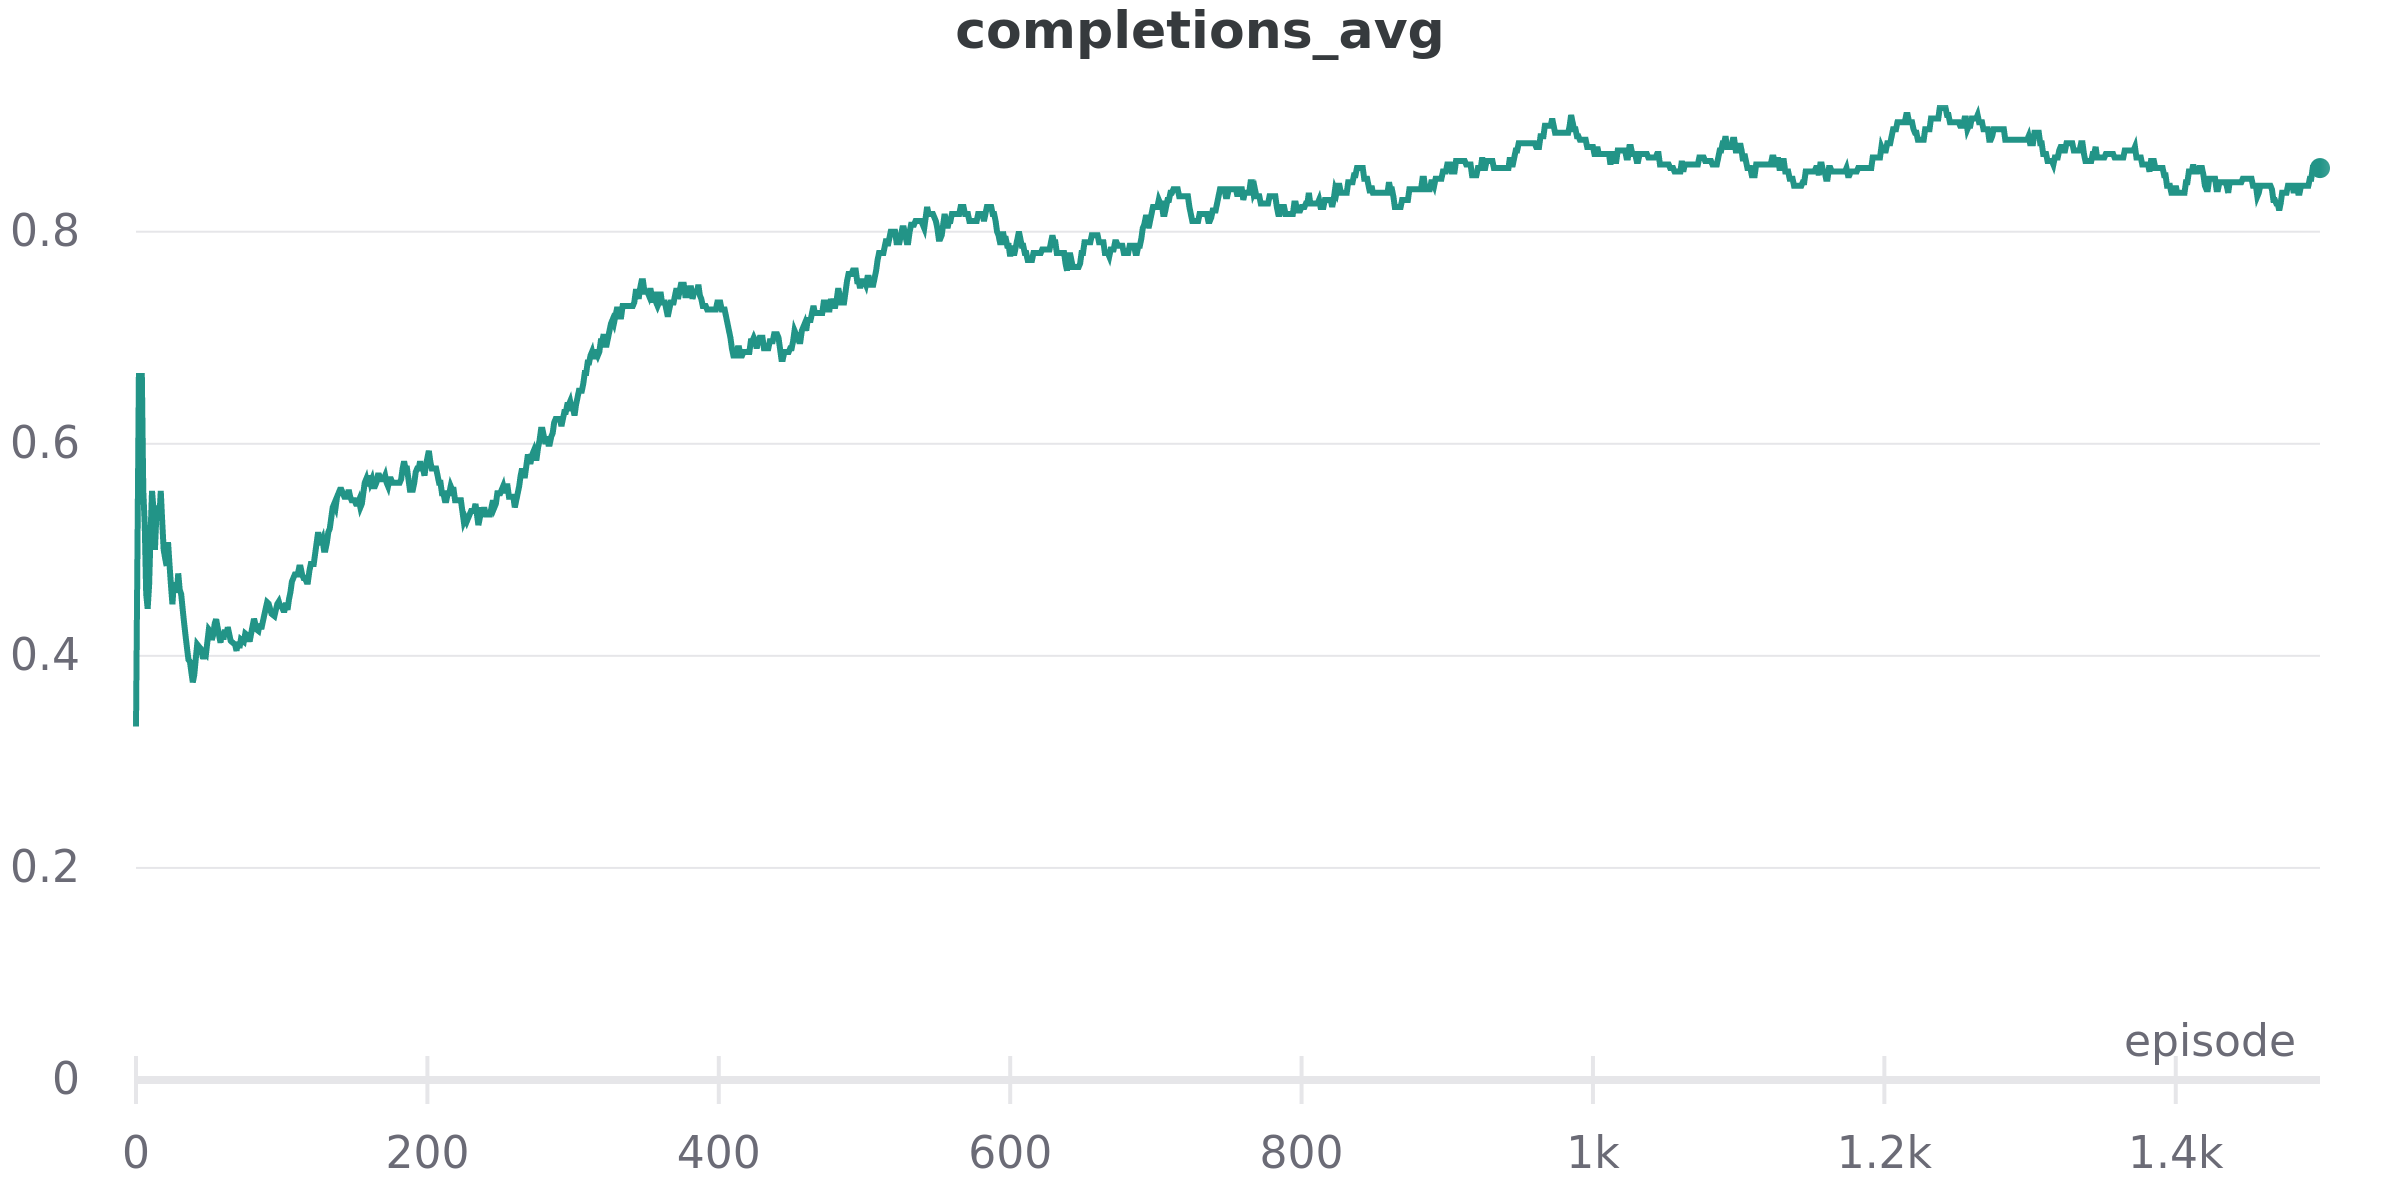
\includegraphics[scale=.2]{res/charts/per_completions.png}}
        \caption{Completions}
\end{figure}

\subsection{Policy Gradients}

TODO Unire policy gradients e actor critic in un solo pezzo?

The policy can be written as $\pi(s)= argmax_aQ(s,a)$ which means that the result of our policy $\pi$, at every state \textit{s}, is the action with the largest Q-value.
The policy is what to look for when solving RL problem. Indeed, when the agent obtains the observation and needs to make a decision, it needs the policy.
In the case where the request is to obtain Q-values, the policy is represented by a neural network that returns values of actions as scalars. 

To be able to obtain those values, the gradient on the policy is computed, which is defined as:
\begin{equation}
    \nabla J \approx \EX[Q(s, a) \nabla \log \pi (a | s) ]
\end{equation}

It follows that the idea is trying to increase the probability of actions that have given good total reward and decrease the probability of actions with bad final outcomes.
On practical view point, policy gradient can be implemented by performing optimization of the following loss function:
\[ \mathcal{L}= -Q(s,a)log \pi(a|s)\]

During SGD the quantity is minimized, therefore there is the minus sign in front of the equation.

The general algorithm of policy gradient methods is synthesized in:
\begin{enumerate}
    \item Initialize the network with random weights;
    \item Play N full episodes, saving their \textit{(s,a,r,s')};
    \item For every step,\textit{t}, of every episode, \textit{k}, compute the discount total reward for subsequent steps: \[ Q_{k,t} = \sum_{i=0} \gamma^i r_i      \]
    \item  Calculate the loss function for all transitions: \[ \mathcal{L}= -\sum_{k,t} Q_{k,t} log( \pi(s_{k,t}, a_{k,t}))\]
    \item Perform an SGD update of weights, minimizing the loss;
    \item Repeat from step 2 until converged.
\end{enumerate}

This preceding algorithm is different from Q-learning one in several aspects: no explicit exploration, no replay buffer, no target network used.
One of the way to improve policy-gradient method, is to reduce the variance of the gradient:
\[var[x] = \EX[(x - \EX[x])^2]\]

If there is a value which has a large variance it could slow down our training significantly cause it may require many samples to \textit{average out} his shift effect. To overcome this problem, it is convenient to subtract the mean total reward from the Q-value, this mean is called \textbf{baseline}.

\textbf{Actor-Critic} method goes further in reducing variance by making the baseline state-dependent, since different states could have very different baselines. The total reward can be represented as a value of the state plus the advantage of the action: $Q(s,a)=V(s)+A(s,a)$. So, using \textit{V(s)} as baseline is not a bad idea, the problem is that \textit{V(s)} is not known. It's possible to use another neural network that will approximate \textit{V(s)} for every observation. To train, it's possible to use the same training procedure that is used in DQN methods. 
When the value (or an approximation) for any state is known, it's possible to use it in order to calculate the policy gradient and update the policy network such that probabilities for actions with good advantage values are increased. The policy network is called \textit{Actor}, since it tells what to do. The other network is called \textit{Critic}, as it allows to understand how good the action were. This improvement is known under the name \textit{Advantage Actor-Critic} (A2C). 

\subsubsection{Proximal Policy Optimization (PPO)}
The core improvement over the basic A2C method is to tweak around the formula used to estimate the policy gradient. The PPO method \cite{ppo} uses as objective function the ratio between the new and the old policy, scaled by the advantages:
\[ J_\theta = E_t[\frac{\pi_\theta(a_t | s_t)}{\pi_{\theta_old}(a_t | s_t)} A_t] \]

To limit the update of the above policy gradient function, it is clipped.
Let's write the ratio between the new and the old policy as:

\[ r_t(\theta) = \frac{\pi_\theta(a_t | s_t)}{\pi_{\theta_old}(a_t | s_t)}\]

Then the clipped objective can be formulated as:

\[J_\theta^{clip} = \EX_t[min(r_t(\theta)A_t, clip(r_t(\theta), 1-\epsilon, 1+\epsilon)A_t)]\]

This new objective limits the ratio between the old and the new policy in the interval $[1-\epsilon, 1+\epsilon]$, so by varying $\epsilon$, size of the update is tuned.

Another substantial difference from A2C method is how the advantage estimation is computed. In classic A2C it's:
\[ A_t = -V(s_t) + r_t + \gamma r_{t+1} + ... + \gamma^{T - t +1} r_{T-1} + \gamma^{T - t}V(s_t)\]
where T are the steps.

In PPO there is a more general estimation:
\[ A_t = \sigma_t + (\gamma \lambda)\sigma_{t+1} + (\gamma \lambda)^2 \sigma_{t+2} + ... + (\gamma \lambda)^{T-t+1}\sigma_{t-1}\]

where $\sigma_t = r_t + \gamma V(s_{t+1})- V(s_t)$. It's possible to notice that the original A2C estimation is a special case of the above one with $\lambda=1$.
Concluding, PPO uses also a long sequence of samples obtained from the environment and then estimate the advantage for the whole sequence before the performance of several epochs of training.

TODO Entropy + decay

TODO Immagine grafici PPO... E se mettessimo quelli che convergono a un'azione?

\subsection{Further Analysis}

\subsubsection{Observation}

TODO Qui la menerei meno sul fatto che con il predictor risolviamo la challenge che è già un miracolo se non uccide tutto

The most effective observation to be used has been noticed to be \textit{TreeObservation}. However, Flatland suggests to find a suitable observation to solve the problems because it is unlikely that the given will be sufficient for the challenge. Our starting point is to extend the \textit{TreeObservation} adding a different predictor.  

The tree observation exploits the fact that a railway network is a graph and thus, the observation is only built along allowed transitions in the graph. The observation is generated by spanning a 4 branched tree from the current position of the agent. Each branch follows the allowed transitions (backward branch only allowed at dead-ends) until a cell with multiple allowed transitions is reached. Here the information gathered along the branch is stored as a node in the tree.

\begin{figure}[H]
\centering
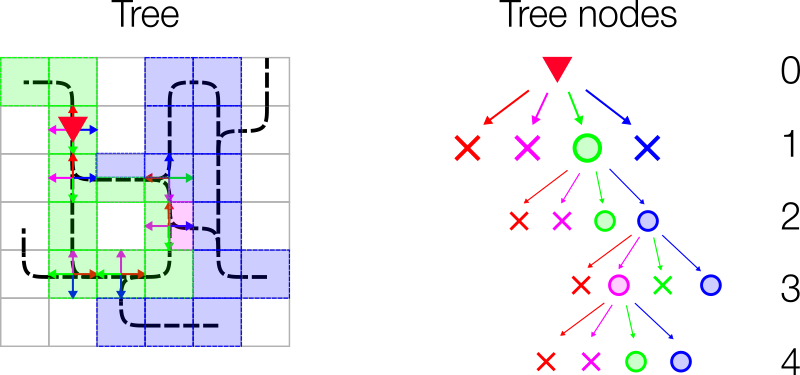
\includegraphics[width=0.6\textwidth]{res/tree_obs.png}
\caption{\label{fig:Views}Tree observation.}
\end{figure}

\subsubsection{Stochastic Path Predictor}
A further help given by the \textit{Flatland RL} library comes from the implementation of a standard \textbf{Predictor}, which could be implemented in the observation to allow the agents to exploit an approximation of the other agent's future positions, helping to prevent deadlocks.

Specifically, this concept is applied in the $4^{th}$ channel of the \textit{TreeObservation}, already provided by the framework. The default predictor, with its basic implementation, assumes every agent to travel through their shortest path.
 
However, this approach results in a simplistic behaviour, since the agents won't always travel along the shortest path. Given the presence of multiple agents and the limited number of tracks, the task of the policy is to put the largest number of agent in the condition to reach the target avoiding deadlocks. This leads agents to choose also longer path in order to try not to block other agents.
 
To overcome this simplification, we decided to add a random factor to the predicted position by implementing a predictor able to guess the agents' future position by sampling from a probability distribution proportional to the distance between the possible paths and the agent's target.

Given a distance $D_{fp}$ between the future position $fp$ and the agent's target and the sum $T$ of distances of all the available paths, the probability of that position to be chosen is given by the following random variable $FP$:
\begin{equation}
P(FP=fp) = \frac{T - D_{fp}}{2 \cdot T}    
\end{equation}

\subsubsection{Deadlock Detection}

Since the agents may present competitive behaviour, it can happen that they lead to a deadlock situation. This happens when an agent cannot perform any action because it is blocked by one or more agents. In a full deadlock situation, no agent will arrive at its own target. This conflict situation is quite common and it increases in frequency proportionally to the number of agents and the dimension of the grid decreasing.
A good point to start with, is to track the deadlocks happening in an episode. In order to do so, for each agent in the environment we check if its \textit{RailAgentStatus} is ``ACTIVE" and if the position in which it has to go is feasible or it is occupied by another agent. Checking if each agent is in deadlock, we return a list of boolean in which \textit{True} means that the agent is in deadlock.

\section{Results}

\subsection{Test Environments}

The proposed solutions have been tested with different environment setups, mainly divided in $N$ levels with growing complexity:

\begin{itemize}
    \item L1: 
        \begin{minted}{javascript}
{
"n_agents": 5,
"x_dim": 20,
"y_dim": 30,
"n_cities": 2,
"max_rails_between_cities": 2,
"max_rails_in_city": 3,
"min_malfunction_interval": 50,
"grid_mode": false,
"malfunction_duration": [20, 50]
}
        \end{minted}
    \item L2: 
        \begin{minted}{javascript}
{
"n_agents": 7,
"x_dim": 30,
"y_dim": 40,
"n_cities": 5,
"max_rails_between_cities": 2,
"max_rails_in_city": 3,
"min_malfunction_interval": 50,
"grid_mode": false,
"malfunction_duration": [20, 50]
}
        \end{minted}
    \item L3: 
        \begin{minted}{javascript}
{
"n_agents": 10,
"x_dim": 40,
"y_dim": 60,
"n_cities": 9,
"max_rails_between_cities": 4,
"max_rails_in_city": 3,
"min_malfunction_interval": 50,
"grid_mode": false,
"malfunction_duration": [20, 50]
}
        \end{minted}
\end{itemize}

TODO Meglio tabella?

\begin{center}
\begin{tabular}{ |c|c| } 
        \hline
    \textbf{Parameter} & \textbf{Value} \\ 
        \hline
    \textcolor{red}{n\_agents} & \textcolor{gray}{10} \\ 
        \hline
    \textcolor{red}{x\_dim} & \textcolor{gray}{40}\\ 
        \hline
    \textcolor{red}{y\_dim} & \textcolor{gray}{60}\\ 
        \hline
    \textcolor{red}{n\_cities} & \textcolor{gray}{9}\\ 
        \hline
    \textcolor{red}{ max\_rails\_between\_cities} & \textcolor{gray}{4}\\ 
        \hline
    \textcolor{red}{max\_rails\_in\_city} & \textcolor{gray}{3}\\ 
        \hline
    \textcolor{red}{min\_malfunction\_interval} & \textcolor{gray}{50}\\ 
        \hline
    \textcolor{red}{grid\_mode} & \textcolor{green}{false}\\ 
        \hline
    \textcolor{red}{malfunction\_duration} & \textcolor{gray}{[20, 50]}\\ 
 \hline
\end{tabular}
\end{center}

\subsection{Hyper-Parameters Tuning}

After all the testing performed, the best set possible of architecture consists of a TODO

The last consists in performing some hyperparameter tuning in order to find the most promising set of parameters for the final training.

TODO Tabella dei parametri 1

TODO Tabella dei parametri 2

We achieved that by performing two different hyperparameters tuning through \hyperlink{https://wandb.ai/}{WandB}: the first one by iterating randomly through a large parameter space and the second by performing a grid search over all the given parameters. The results are the following. 

By considering the completions percentage (TODO o meglio l'average score?) we could infer the optimals parameters for the DDDQN architecture.

TODO Tabella parametri finali

\subsubsection{Performances}

TODO Qui potremmo runnare su un 100aio di episodi per ogni env la rete definitiva con il training disattivato

\section{Conclusions}

\subsection{Future Work}

\subsubsection{Hindsight Experience Replay}

A first improvement which would probably \cite{her}.

Store the replay buffer, the original goal and a new subset of other goals after each episode. Therefore even from a failed attempt, a positive reward can be obtained.
This new goals can be chosen using 4 different strategies:
\begin{enumerate}
    \item Final: The new goals is the goal achieved in the final state of the episode
    \item Future: Replay with k random states which come from the same episodes as the transition being replayed and were observed after it.
    \item Episode: Replay with k random states coming from the same episodes as the transition being replayed
    \item Random: Replay with k random states encountered so far in the whole training procedure.
\end{enumerate}

\subsubsection{Truly Proximal Policy Optimization}

A PPO improvement \cite{truly-ppo}.

TODO Non so cosa sia ma potrebbe essere messo come miglioramento del PPO

\subsubsection{Trust Region-Guided Proximal Policy Optimization}

Another PPO improvement \cite{trgppo}.

TODO Come sopra

\newpage

\printbibliography

\end{document}